\chapter{Experiments} \label{chap-5}

[Grammar is unchecked...]
This chapter presents the results of initial experimental studies of elliptical painting at the SNS. The simulations in chapter \ref{chap-2}-\ref{chap-3} were used to guide the experiments, and the diagnostics described in chapter \ref{chap-4} were used to measure the painted distribution. Recall from chapter \ref{chap-3} that solenoid magnetic fields should help the distribution remain close to a Danilov distribution during injection; solenoid magnets were planned to be installed in the SNS ring in 2021, but their installation was delayed until mid-2022, outside the dogmatic of this dissertation. Thus, the beams created in the following experiments were not expected to be optimal. Nonetheless, it was hoped that the beams would be clearly distinguishable from a production beam produced by correlated painting. 


\section{Experimental procedure}

Accelerator physics experiments are performed in the SNS control room using the OpenXAL framework. OpenXAL provides a high-level interface to perform tasks such as changing magnet strengths, triggering the beam, etc. It can also perform single-particle or envelope tracking using an online model of the accelerator. OpenXAL scripts are written in Java or Jython and are executed from the command line. Many graphical user interface (GUI) OpenXAL applications have been developed over the history of the SNS and are available for use in the control room. 

The following steps are taken during the experimental setup:
%
\begin{enumerate}
    \item 
    The beam energy is lowered from 1.0 GeV to 0.8 GeV by turning off several RF cavities at the end of the linac. This is performed by the SNS operations team. Generally, lowering the energy causes other accelerator components to trip or malfunction due to the modified timing system; these must be corrected one-by-one. The first attempt to lower the energy to 0.8 GeV took over six hours.
    %
    \item
    The horizontal and vertical tunes are set to the same value using the Ring Optics Control (ROC) application. ROC varies several quadrupoles until the model tunes are equal to the desired tunes. The tunes are measured using turn-by-turn BPM readings from a single minipulse in the ring. Generally, the measured and model tunes are not quite equal; we therefore shift the ROC input tunes until they agree with the measured tunes. The measured tunes are assumed to be accurate to at least two decimal places.
    %
    \item
    (Optional: Modify the injection region in some way to increase the effective kicker strength.)
    %
    \item
    The eight injection kicker magnets are calibrated using the Ring Injection Control (RIC) application, as described in chapter \ref{chap-1}. 
    %
    \item
    The initial/final kicker voltages are determined to obtain the desired closed-orbit coordinates at the foil, as described in \ref{chap-1}.
    %
    \item
    The initial/final voltages are connected with a square root waveform; the waveform is applied to the injection kickers. The duration of the waveform — the painting time — is chosen at this step but can be easily changed later on. The painting time determines the number of minipulses in the final distribution; i.e., the beam intensity.
    %
    \item
    The number of injected turns before extraction is chosen. This allows the distribution to be measured at different times during injection.  It is also possible to store the beam in the ring, although the SNS normally extracts the beam immediately after accumulation.
    %
\end{enumerate}
%
The next task is to prepare for the measurements. For the wire-scanner measurement, the first step is to modify the RTBT optics using the application developed as part of this dissertation. If the fixed-optics method is used, the optics are changed immediately. If the multi-optics method is used, the optics are pre-computed and stored for later use. The SNS employs a sophisticated machine protection system (MPS) that will cause the machine to trip if the RTBT quadrupole strengths wander outside a certain window, so this window is extended beforehand. Additionally, MPS will activate if the fractional change in field strength is too large; to solve this problem, the field strength is changed in small steps. Wire-scanner data acquisition is performed by the Profile Tools and Analysis (PTA) application. The beam is set to a pulse frequency of 1 Hz, and the beam loss monitors in the wire-scanner region are masked due to the higher-than-normal losses when the wires cross the beam core. After the four wire-scanners complete their scan, a time-stamped file containing the measured profiles along with their statistical properties (mean, standard deviation, etc.). 

The second measurement is the tomographic reconstruction from $x$-$y$ projections on the target. Since the optics calculation is time-consuming, it is generally run in the background while wire-scans are collected; the quadrupole strengths are saved to a file. Since the use the target images for tomographic reconstruction was proposed late in this research, the target scan was only performed in the last of the following experiments.


\section{Experiment 1}

The SNS reserves approximately one day per month for accelerator physics experiments, and various experiments must compete for time within this twenty-four hour period. At the time of our first experiment, setup of the injection region using the RIC application had not yet been completed; although simulations indicated that the kickers were not strong enough to perform elliptical painting at 1 GeV kinetic energy, this had not been tested in reality. And the SNS energy had not yet been decreased — a time-consuming and possibly error-prone task. The goal of Experiment 1 was therefore to push the injected coordinates $x$ and $y'$ to their limits at 1 GeV.

Simulations predict that the distribution will undergo significant change during injection, especially without the presence of solenoid magnets in the ring; therefore, it is interesting to measure the distribution not only at its final state, but also at the intermediate states. Using the fixed-optics method, ten measurements can be performed within one hour. 

\subsection{Correlated painting}

Before setting up for elliptical painting, a production beam was measured for comparison. Recall that a production beam is produced using correlated painting: the displacements at the foil are increased from an initial offset to their final value, and the slope at the foil is always zero. The number of injected turns was reduced from 1000 to 500, and the beam was measured every 50 turns. The measured wire-scanner profiles are shown in Fig.~\ref{fig:exp1a_wsmeas}.
%
\begin{figure}[!p]
    \centering
    \begin{subfigure}{\textwidth}
        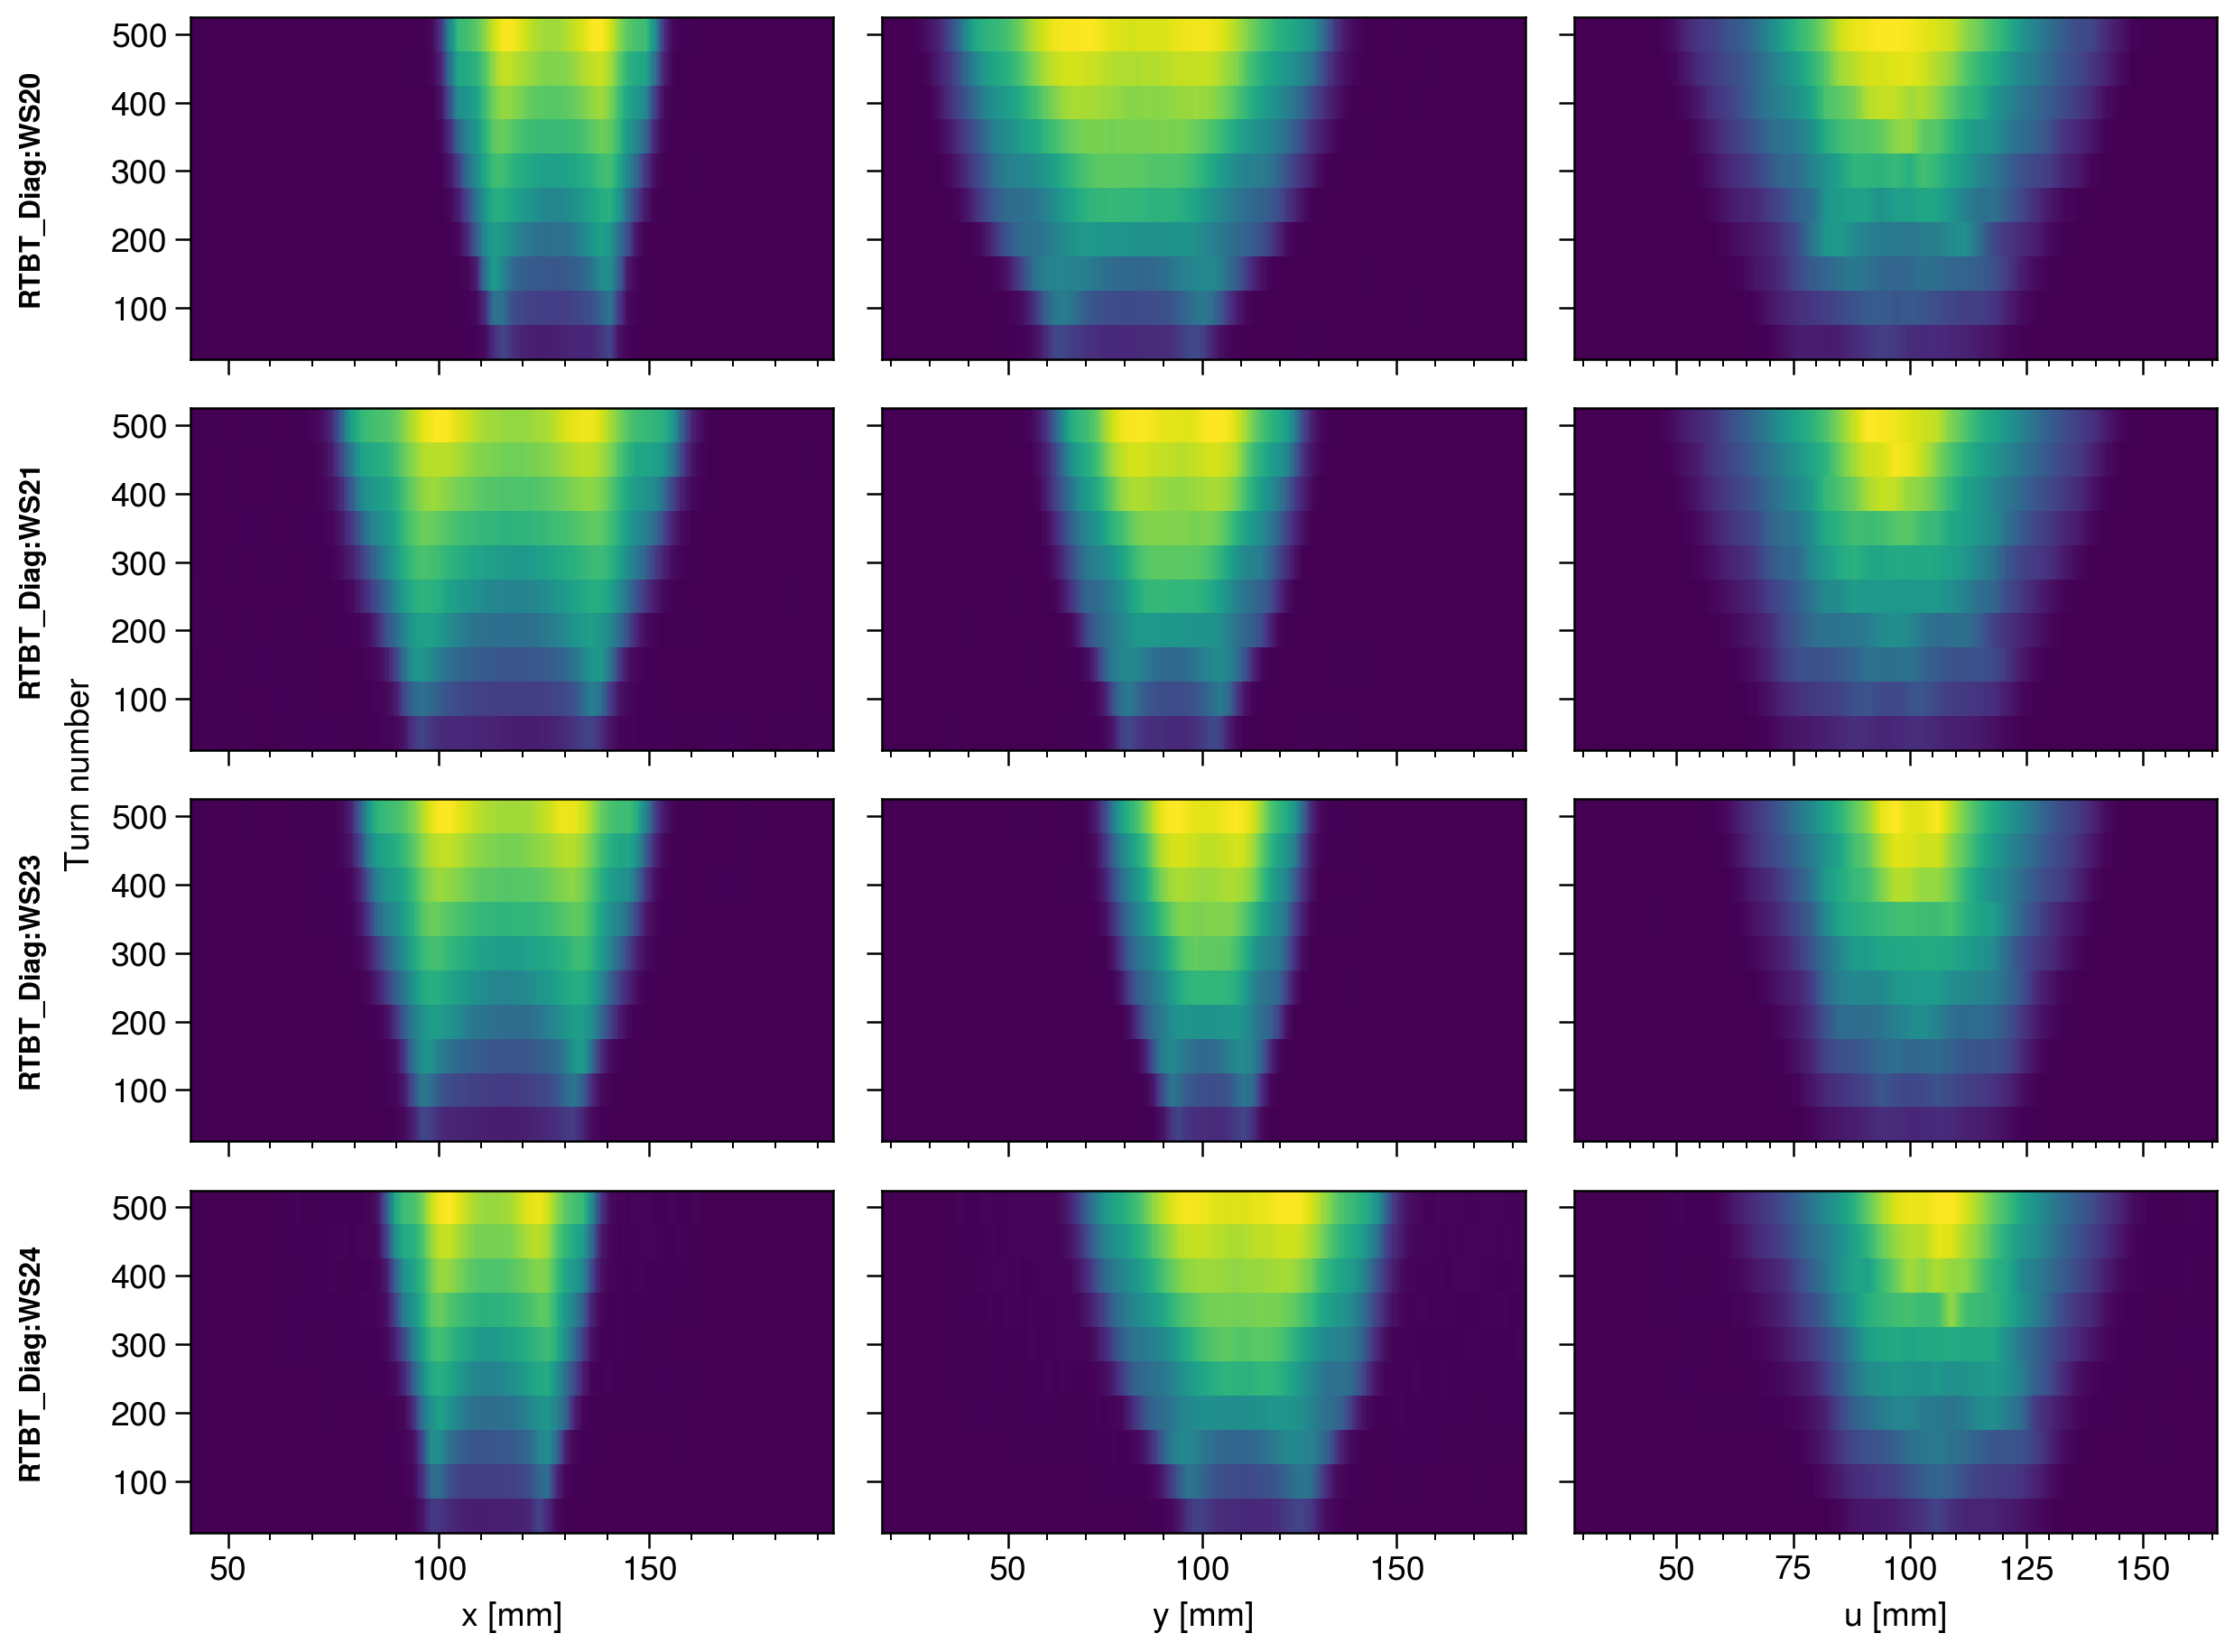
\includegraphics[width=\textwidth]{Images/chapter5/exp1a/waterfall.png}
    \end{subfigure}
    \vfill
    \vspace*{1.25cm}
    \vfill
    \begin{subfigure}{\textwidth}
        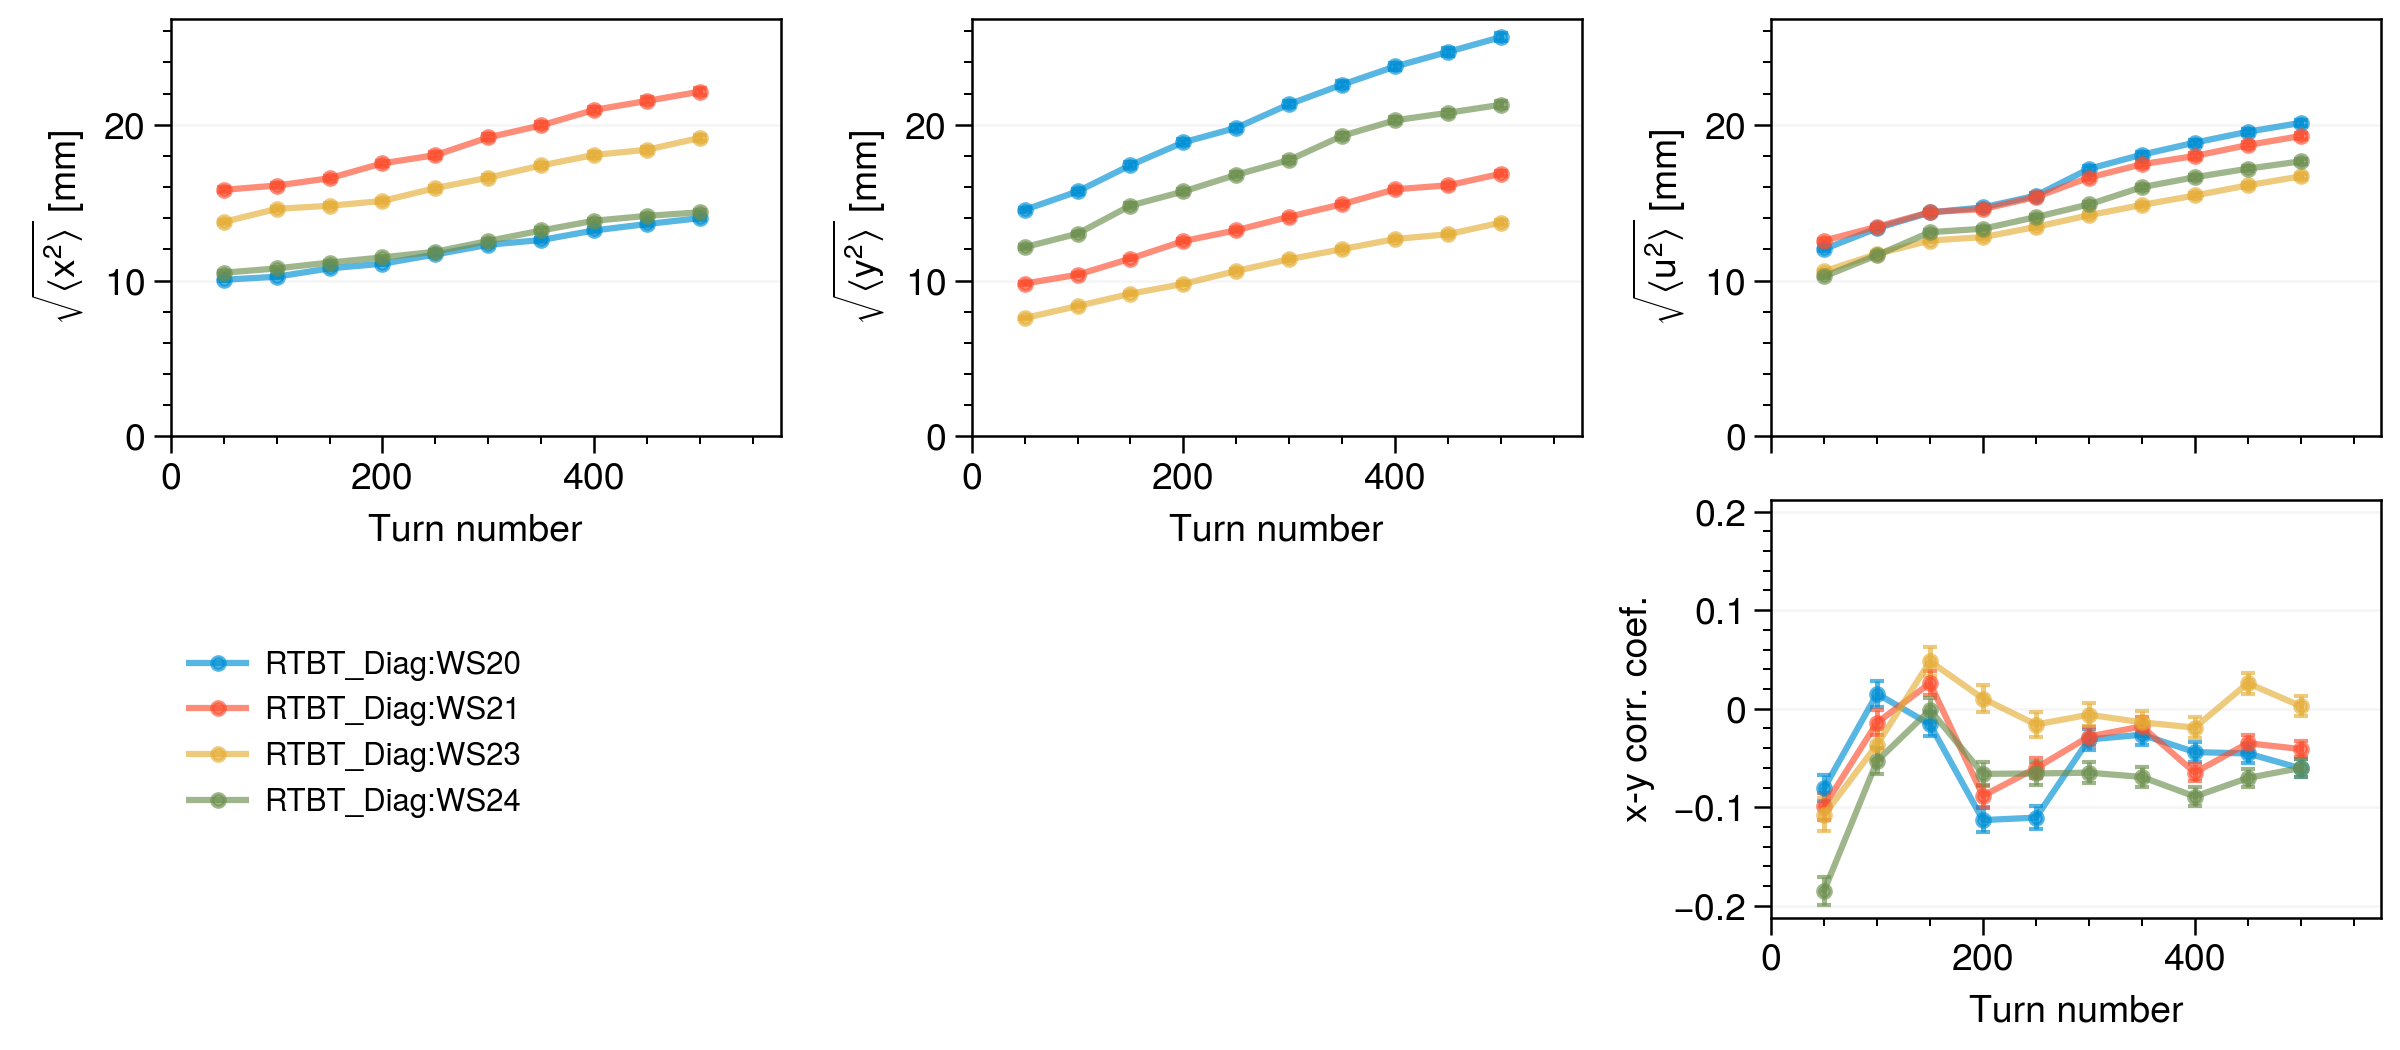
\includegraphics[width=\textwidth]{Images/chapter5/exp1a/rms.png}
    \end{subfigure}
    \caption{Measured wire-scanner profiles during injection for a 1 GeV production beam, 500 injected turns.}
    \label{fig:exp1a_wsmeas}
\end{figure}
%
Each subplot shows the evolution of the projection onto a single wire during injection; each row corresponds to a different wire-scanner and each column corresponds to a different projection axis — $x$, $y$, $u$. That the closed orbit starts offset from the foil is evident from initial two peaks in the $x$ and $y$ projections. The distribution forms a ring or donut in $x$-$x'$ and $y$-$y'$. The hollow center eventually becomes partially filled due to space charge and other nonlinear effects.


%
\begin{figure}[!p]
    \centering
    \begin{subfigure}{0.6\textwidth}
        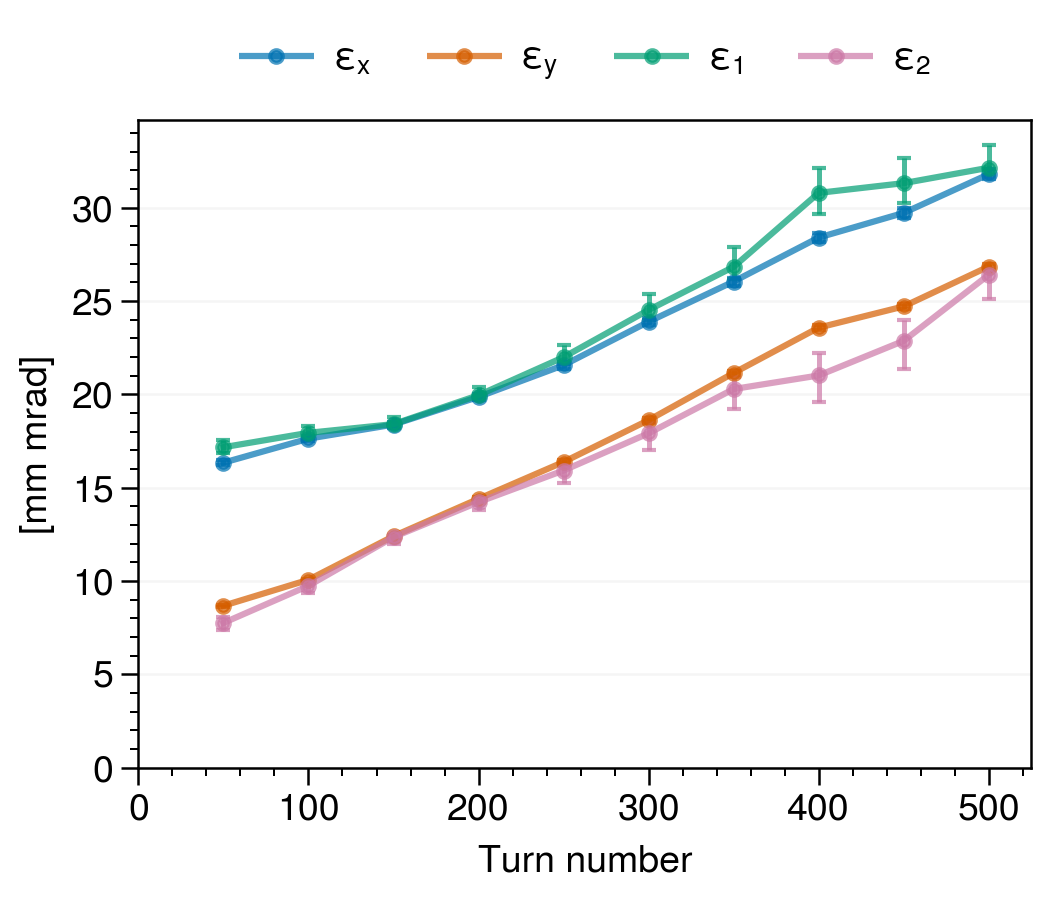
\includegraphics[width=\textwidth]{Images/chapter5/exp1a/emittances.png}
    \end{subfigure}
    \vfill
    \vspace*{0.0cm}
    \vfill
    \begin{subfigure}{0.8\textwidth}
        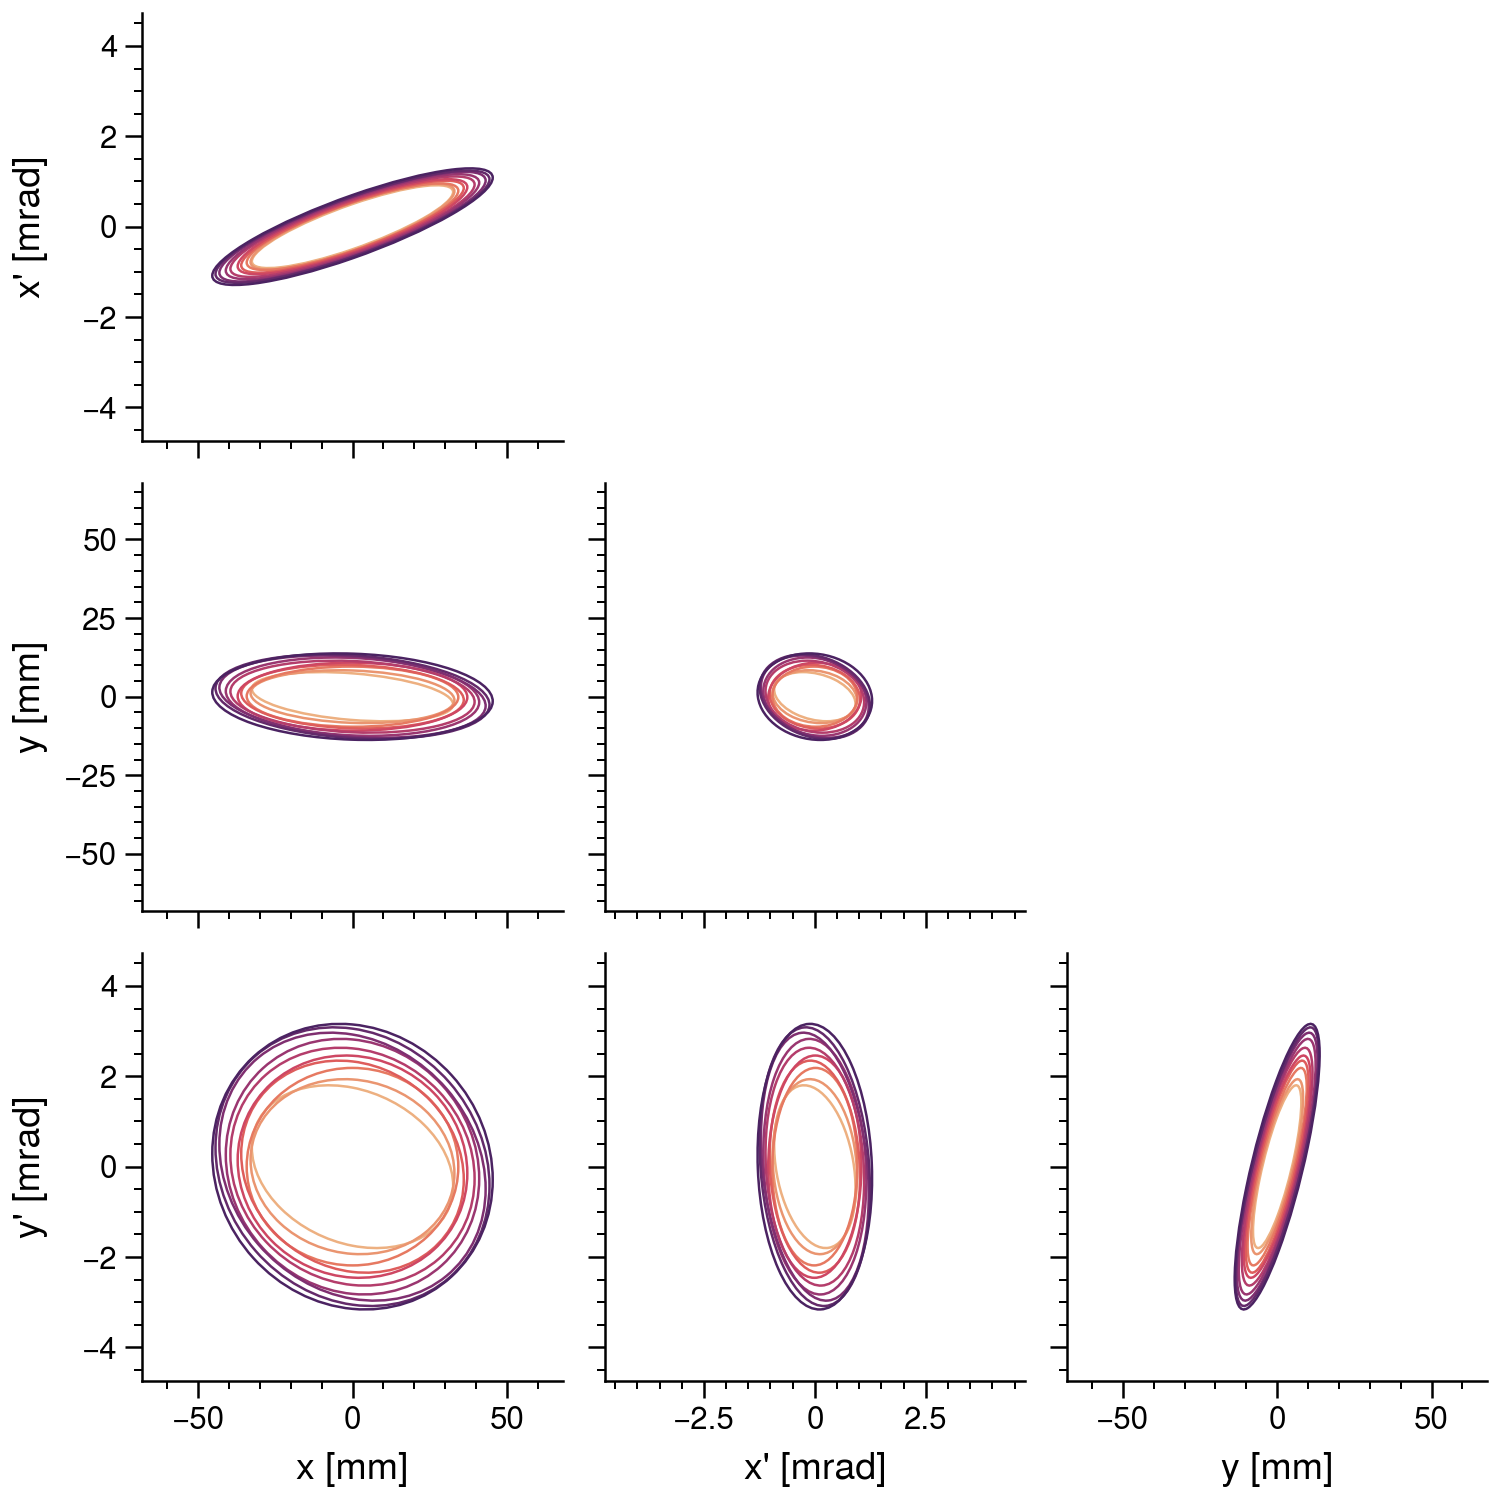
\includegraphics[width=\textwidth]{Images/chapter5/exp1a/corner.png}
    \end{subfigure}
    \caption{Reconstructed emittances and covariance ellipses of a 1 GeV production beam during injection (500 turns). In this and subsequent figures, light/dark ellipses correspond to the start/end of injection.}
    \label{fig:exp1a_emittances}
\end{figure}
%



\subsection{Elliptical-ish painting}

[... We should probably show some screenshots of the RIC application. Maybe not here, but somewhere. ...]

%
\begin{figure}[!p]
    \centering
    \begin{subfigure}{\textwidth}
        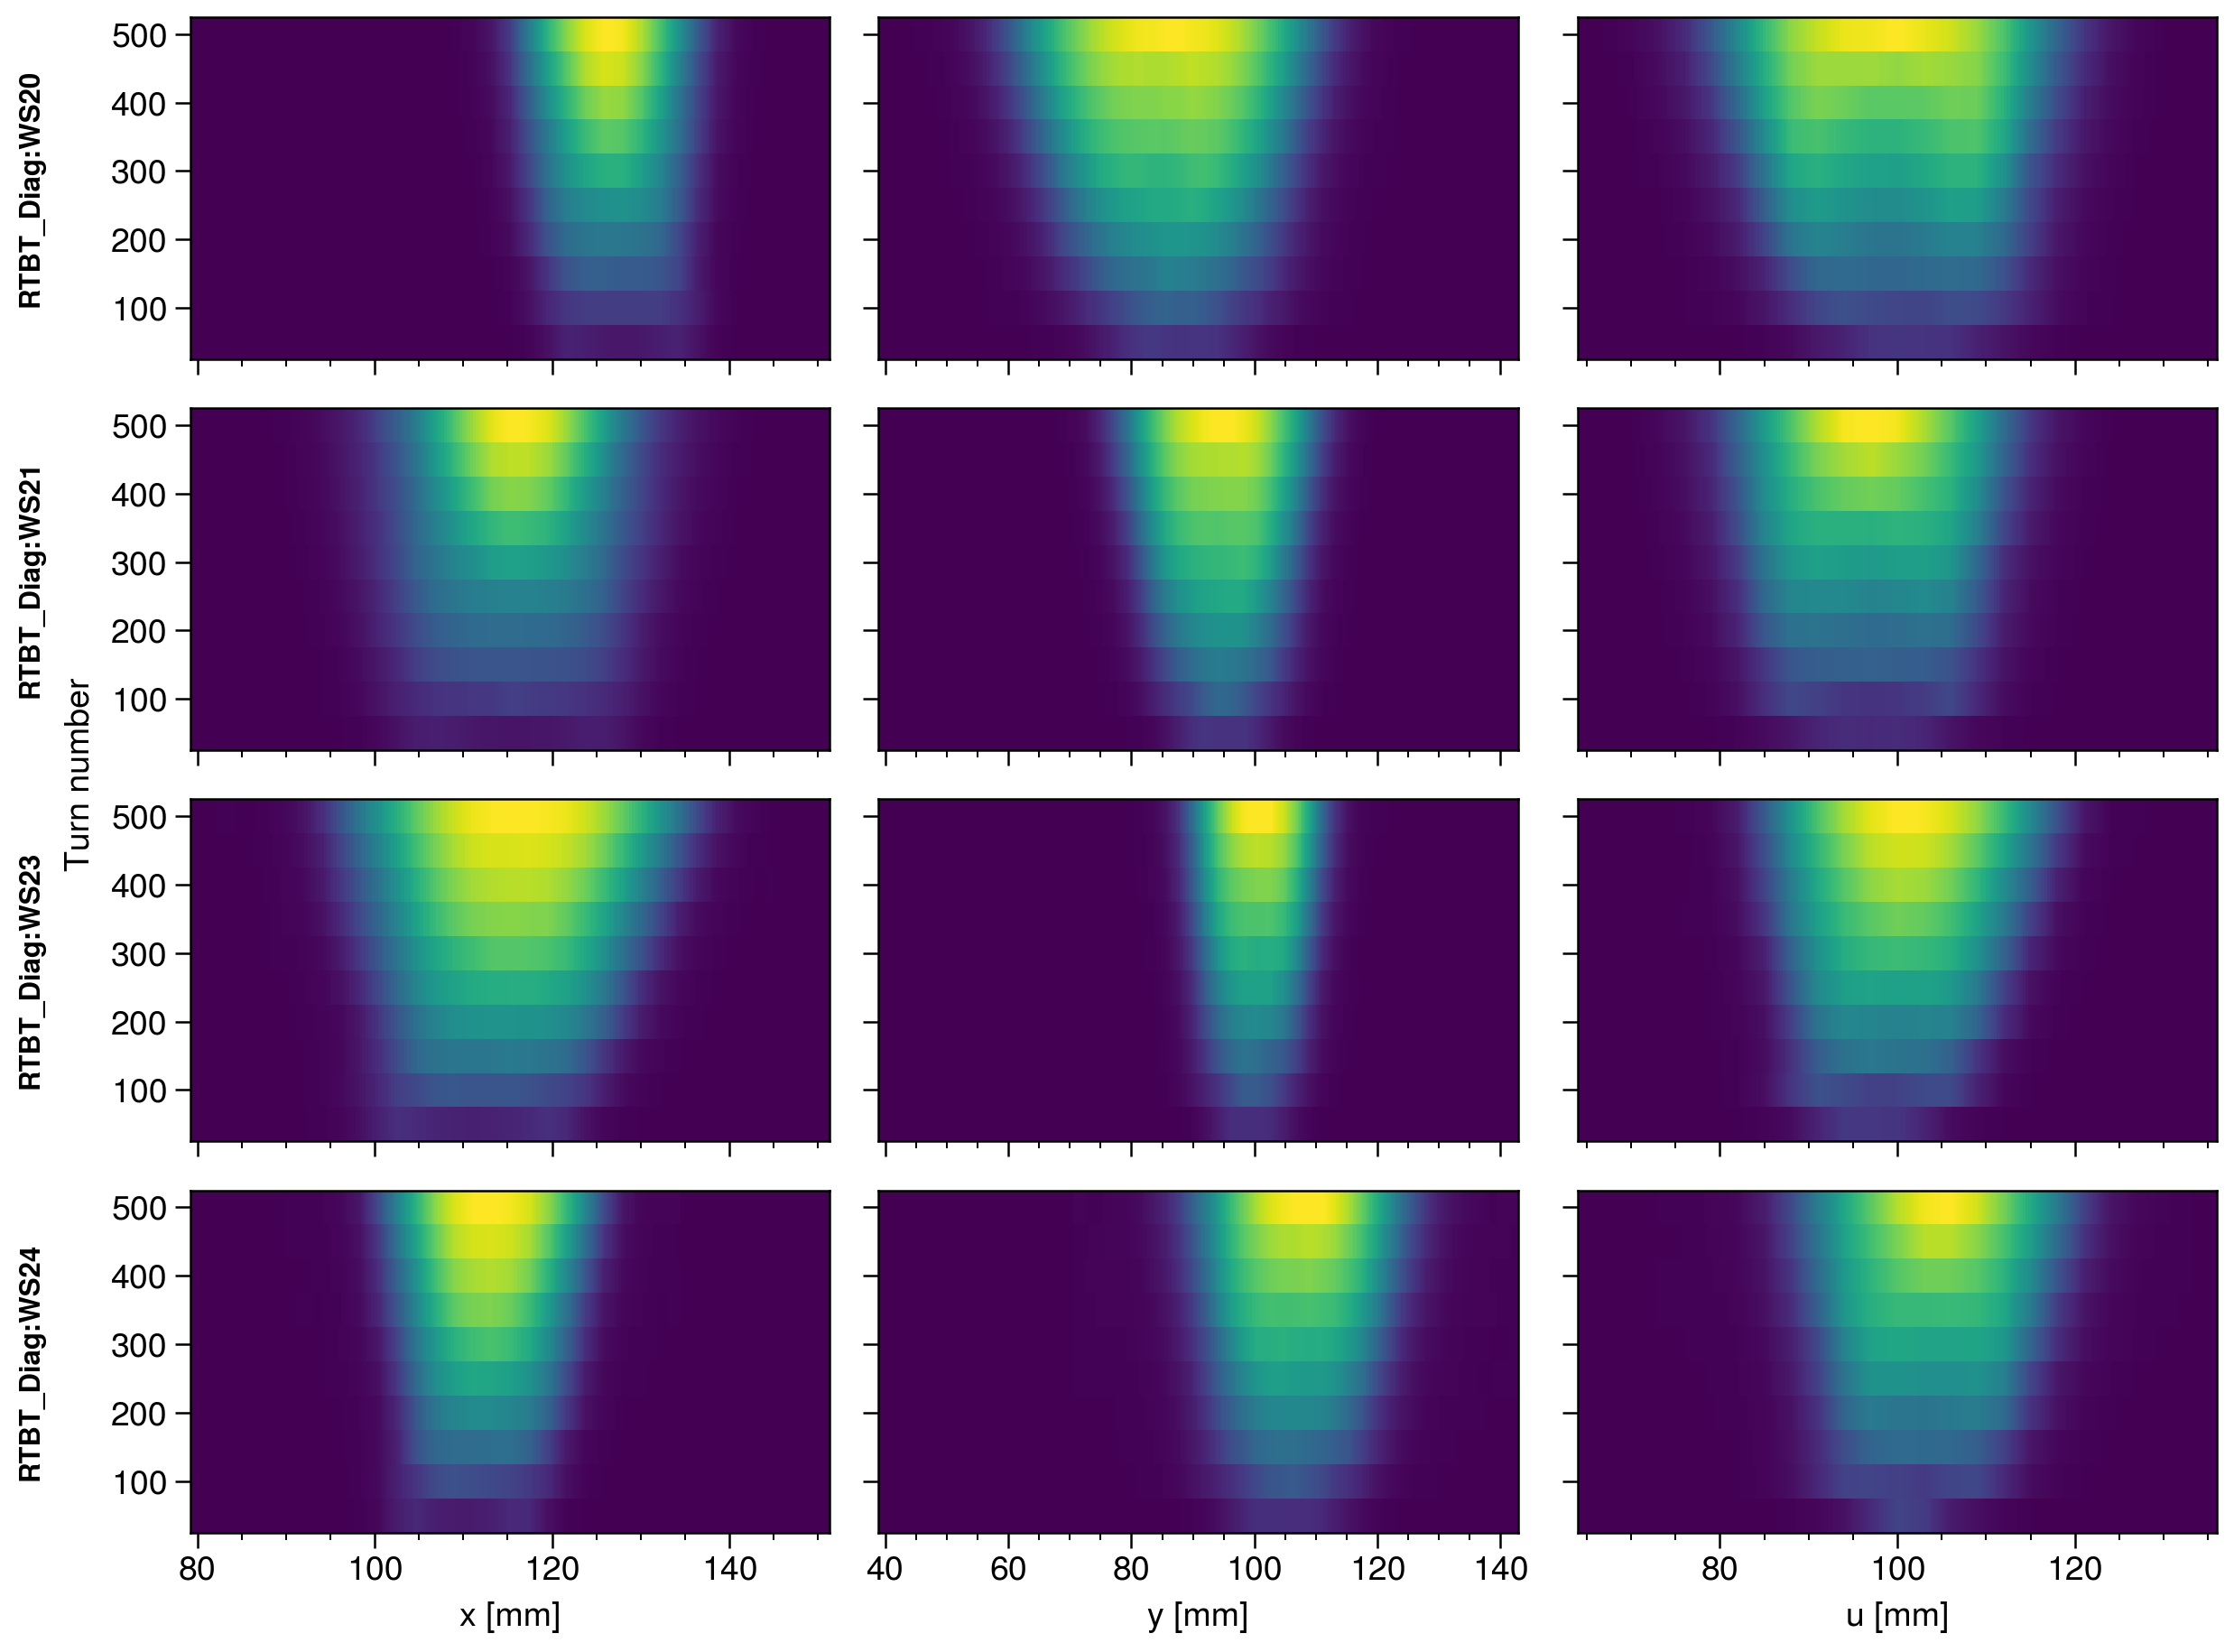
\includegraphics[width=\textwidth]{Images/chapter5/exp1b/waterfall.png}
    \end{subfigure}
    \vfill
    \vspace*{1.25cm}
    \vfill
    \begin{subfigure}{\textwidth}
        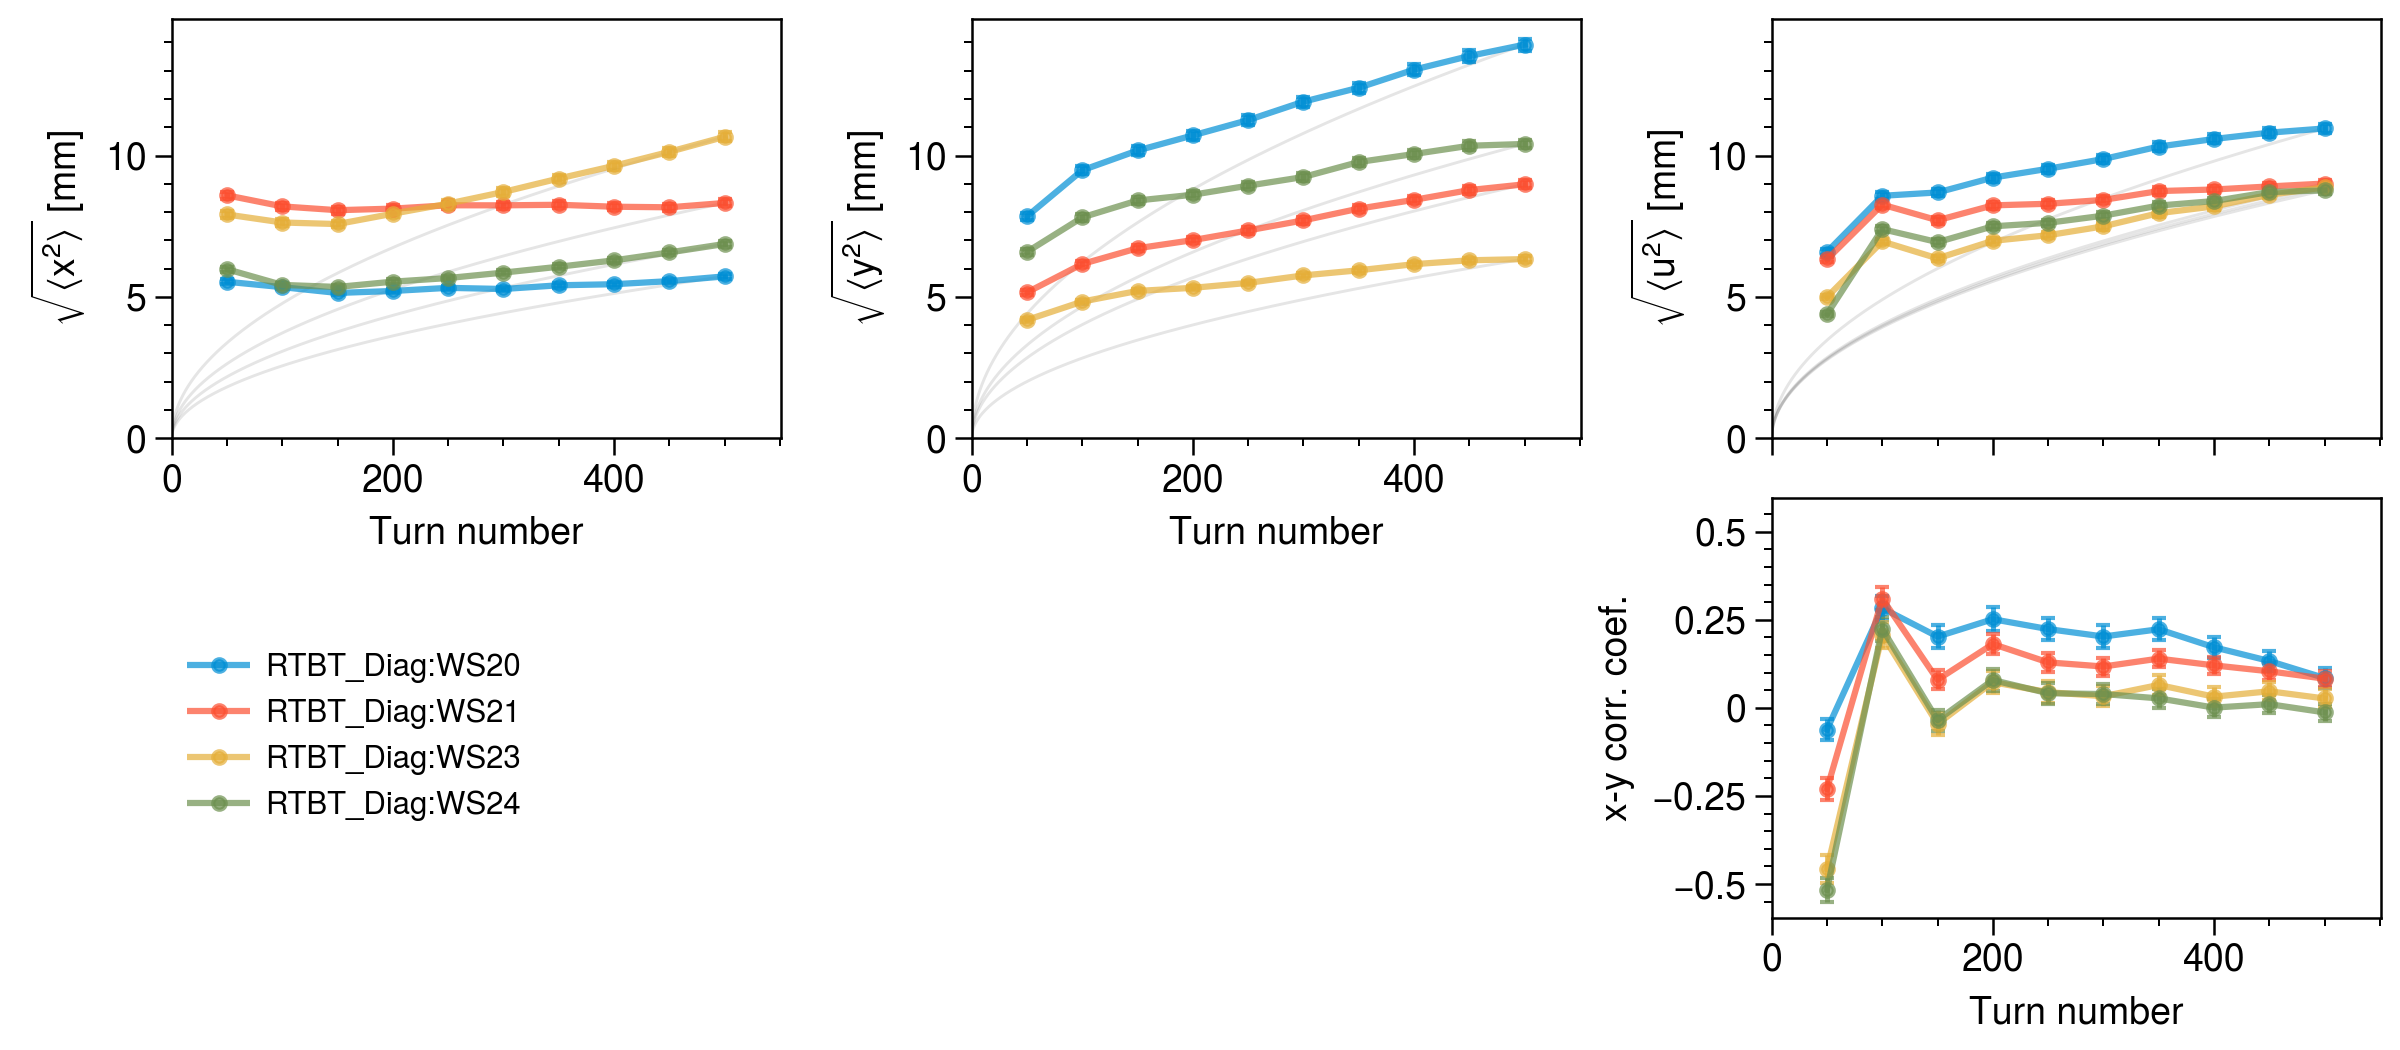
\includegraphics[width=\textwidth]{Images/chapter5/exp1b/rms.png}
    \end{subfigure}
    \caption{Measured wire-scanner profiles during injection for a 1 GeV beam. Initial injected coordinates: ($x$, $x'$, $y$, $y'$) $\approx$ (10 mm, 0 mrad, 0 mm, 0 mrad). Final injected coordinates: ($x$, $x'$, $y$, $y'$) $\approx$ (21 mm, 0 mrad, 0 mm, 0.7 mrad).}
    \label{fig:exp1b_wsmeas}
\end{figure}
%

%
\begin{figure}[!p]
    \centering
    \begin{subfigure}{0.6\textwidth}
        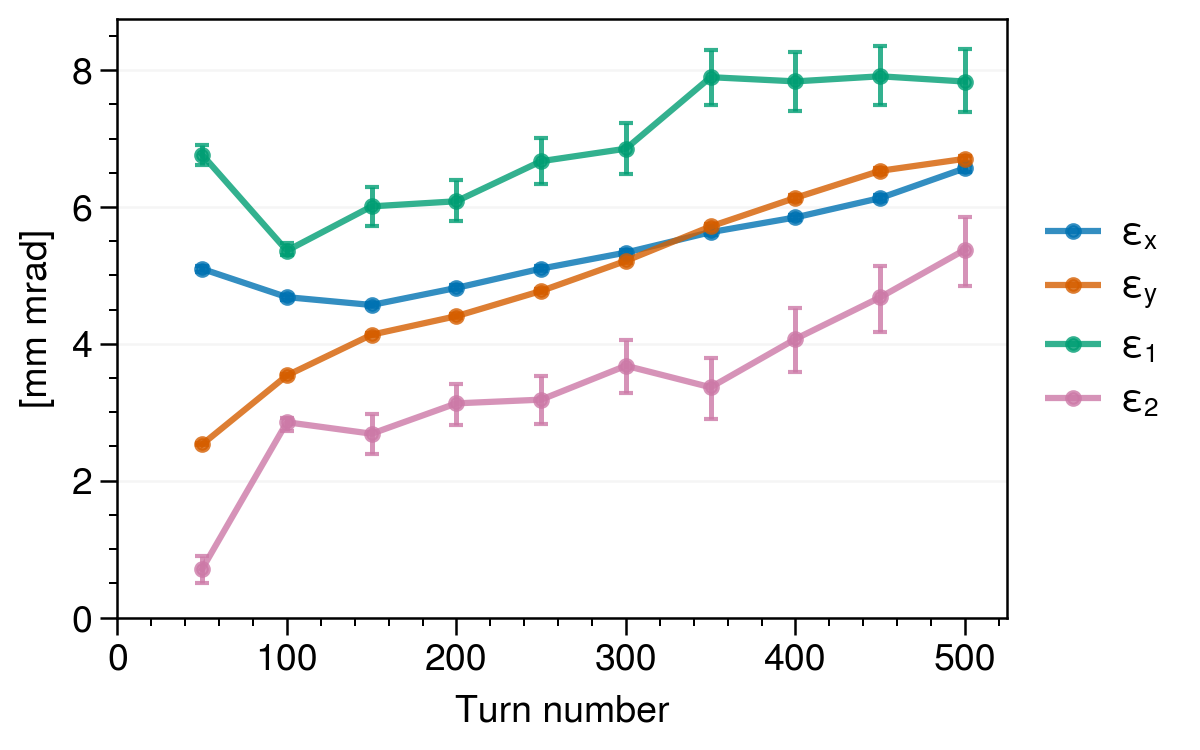
\includegraphics[width=\textwidth]{Images/chapter5/exp1b/emittances.png}
    \end{subfigure}
    \vfill
    \vspace*{-0.2cm}
    \vfill
    \begin{subfigure}{0.8\textwidth}
        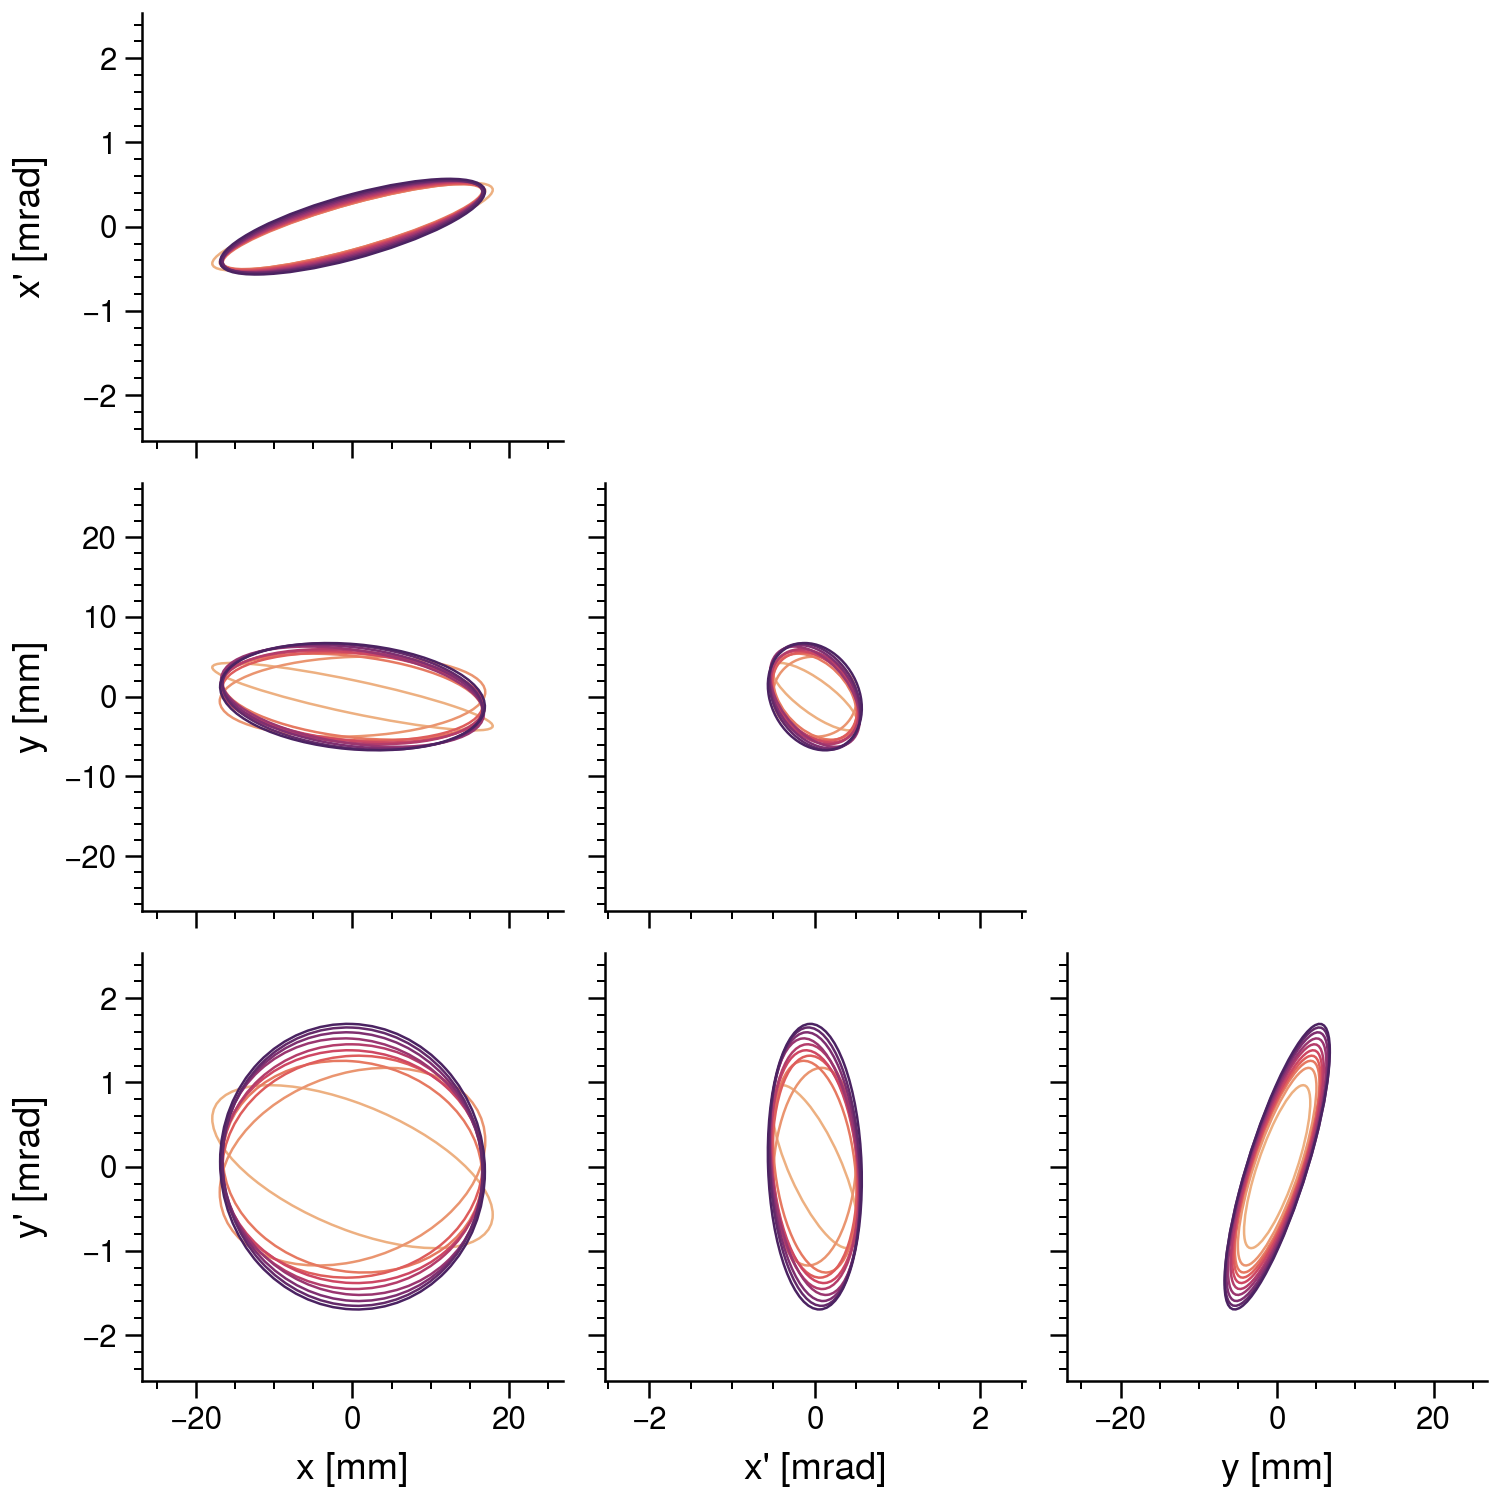
\includegraphics[width=\textwidth]{Images/chapter5/exp1b/corner.png}
    \end{subfigure}
    \caption{Reconstructed emittances and covariance ellipses for a 1 GeV beam. Initial injected coordinates: ($x$, $x'$, $y$, $y'$) $\approx$ (10 mm, 0 mrad, 0 mm, 0 mrad). Final injected coordinates: ($x$, $x'$, $y$, $y'$) $\approx$ (21 mm, 0 mrad, 0 mm, 0.7 mrad).}
    \label{fig:exp1b_emittances}
\end{figure}
%


\section{Experiment 2}

[... Mention failed attempt to optimize the orbit corrector dipoles in the injection region. ...]

%
\begin{figure}[!p]
    \centering
    \begin{subfigure}{\textwidth}
        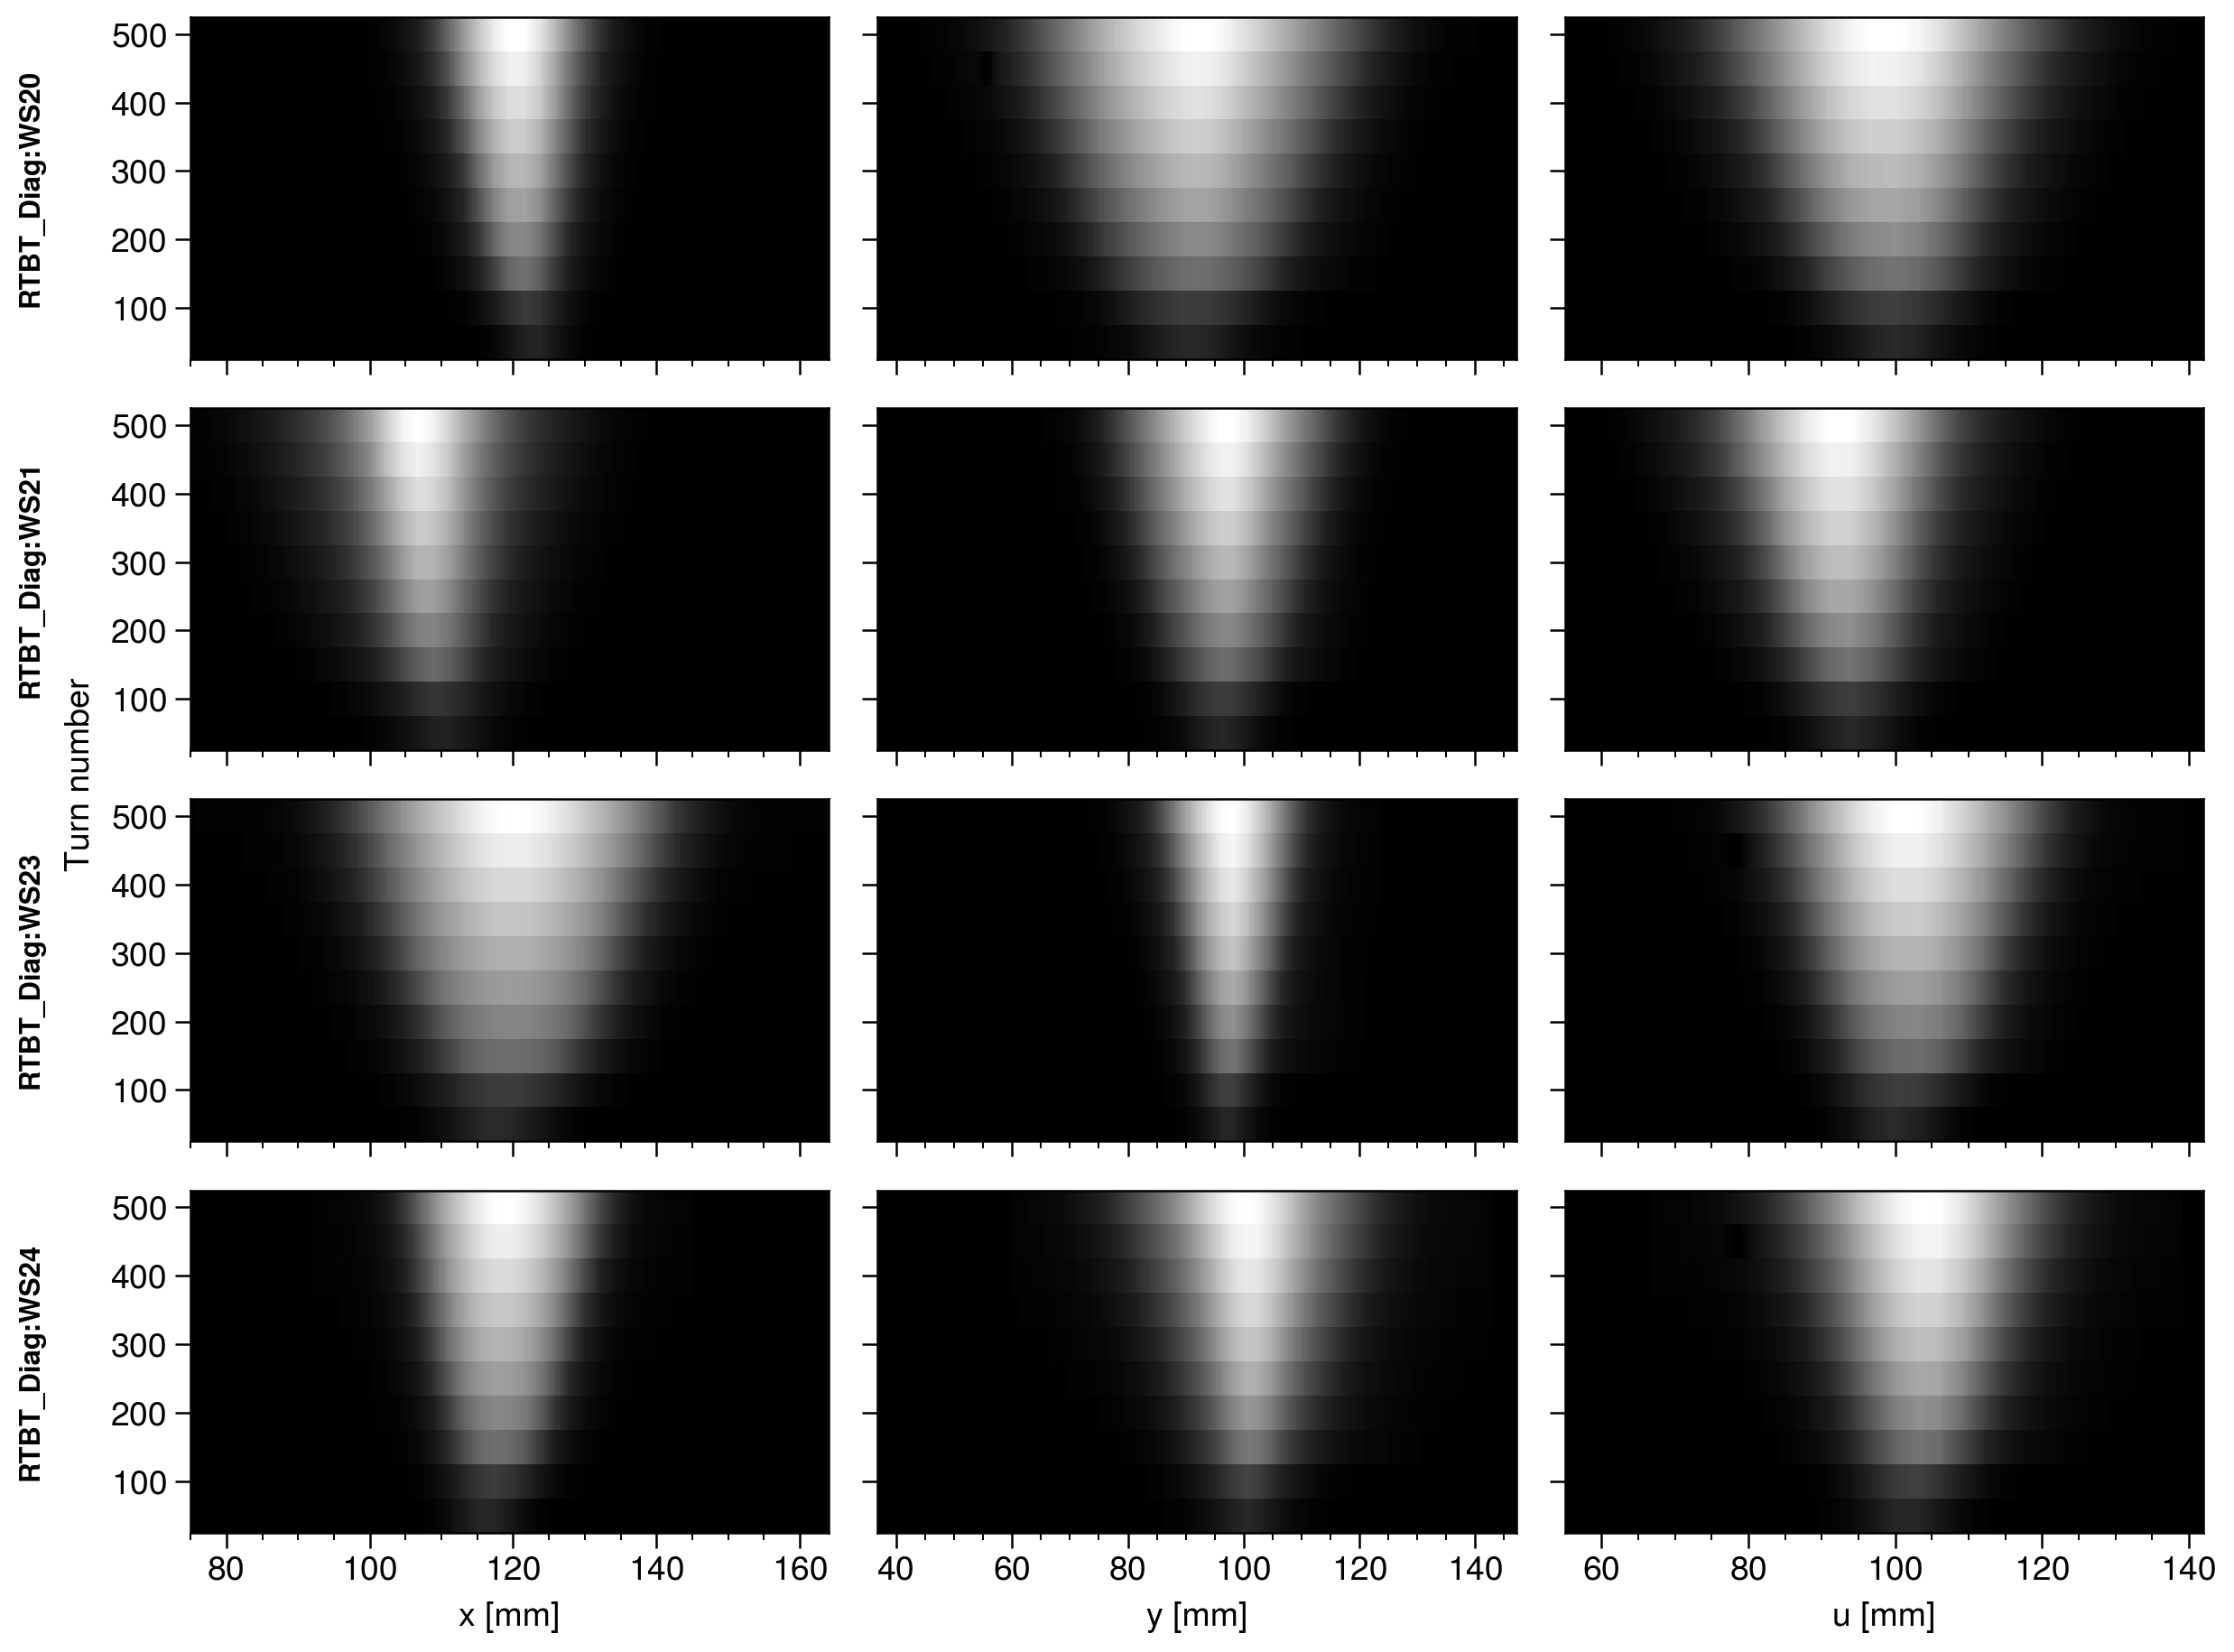
\includegraphics[width=\textwidth]{Images/chapter5/exp2/waterfall.png}
    \end{subfigure}
    \vfill
    \vspace*{1.25cm}
    \vfill
    \begin{subfigure}{\textwidth}
        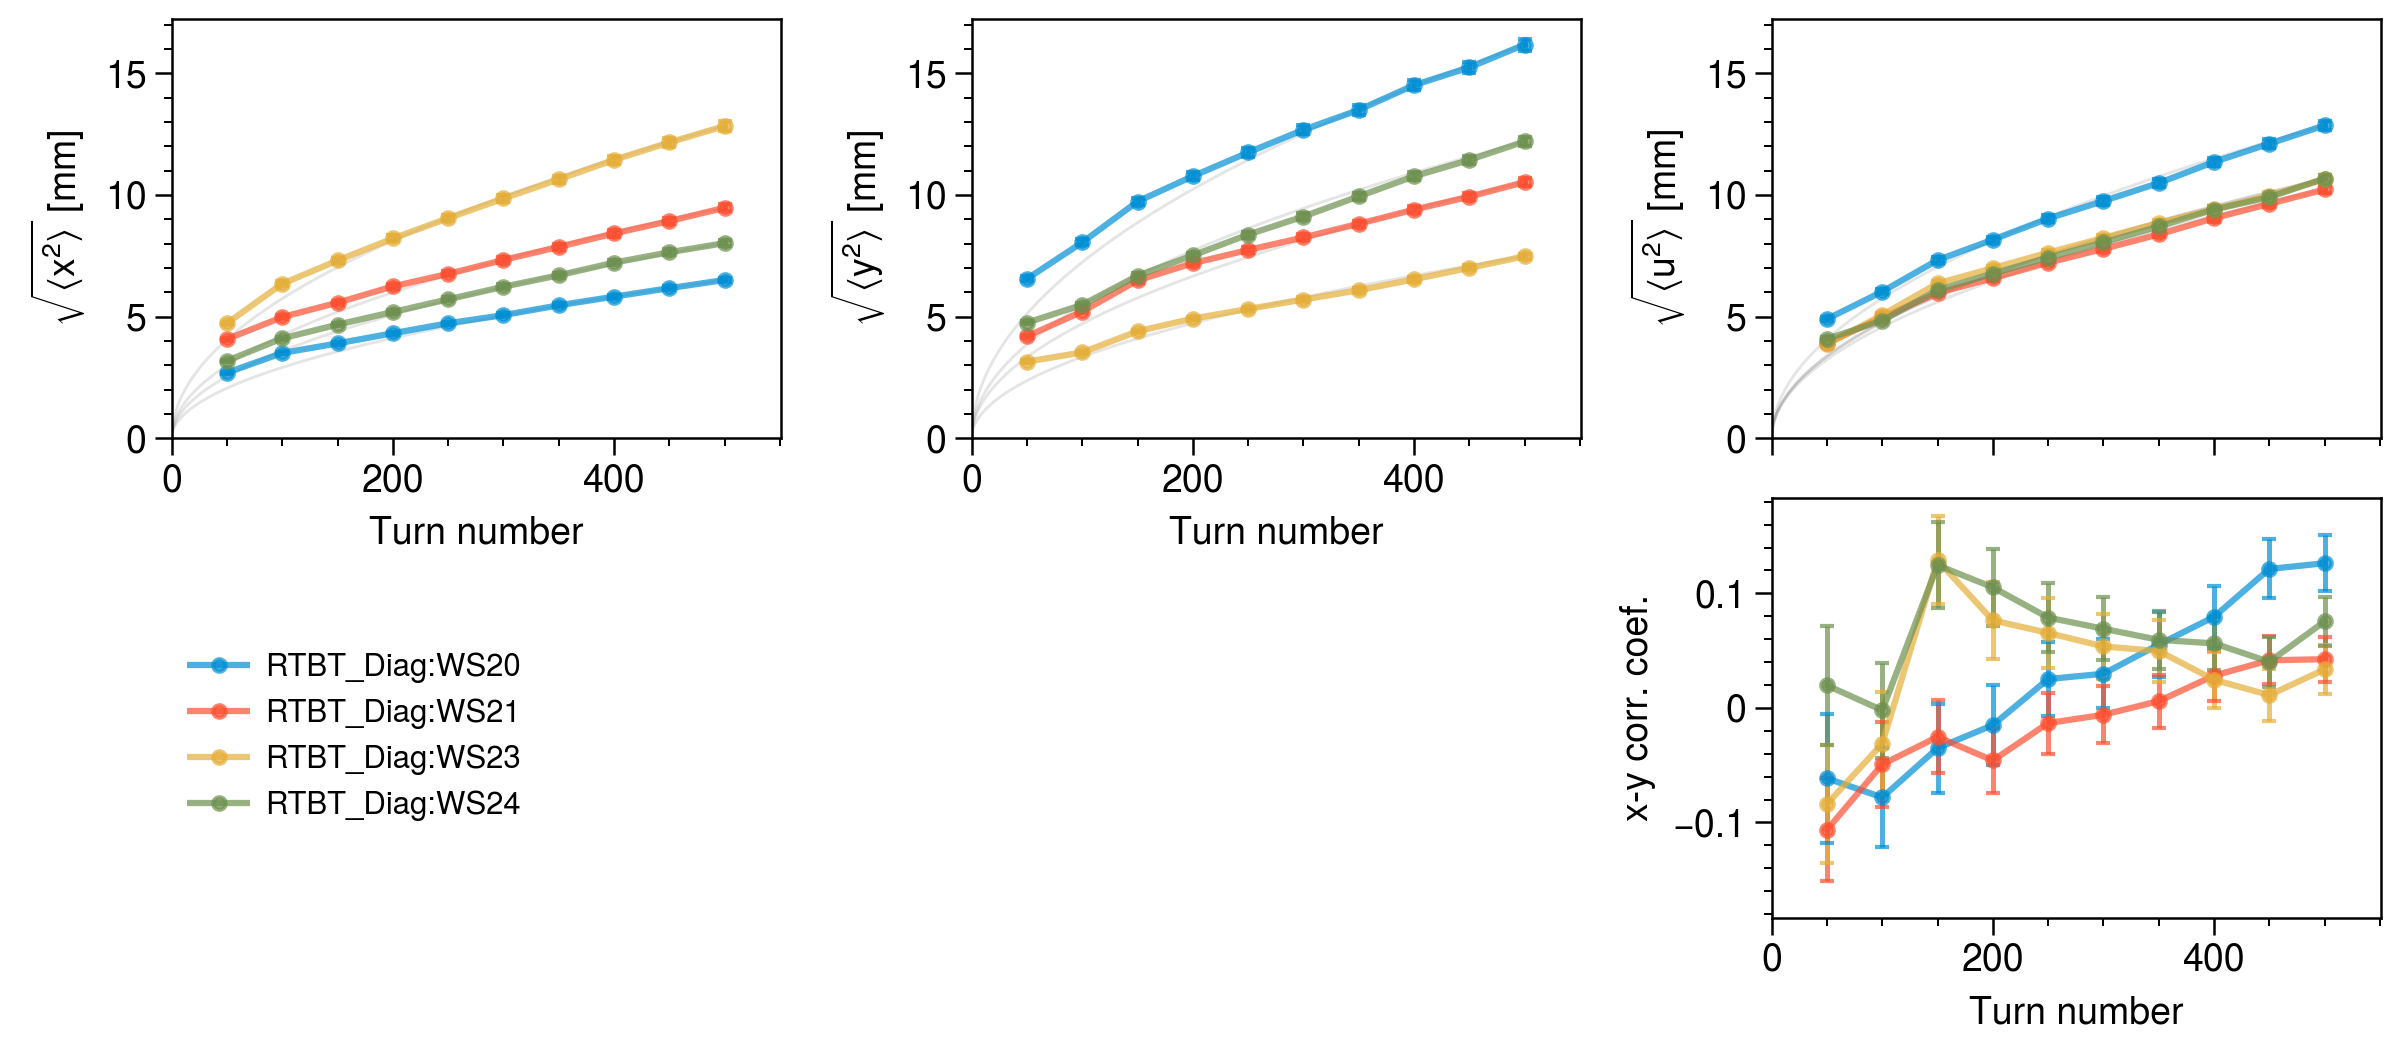
\includegraphics[width=\textwidth]{Images/chapter5/exp2/rms.png}
    \end{subfigure}
    \caption{Measured wire-scanner profiles during injection for a 0.8 GeV beam. Initial injected coordinates: ($x$, $x'$, $y$, $y'$) $\approx$ (0 mm, 0 mrad, 0 mm, 0 mrad). Final injected coordinates: ($x$, $x'$, $y$, $y'$) $\approx$ (21 mm, 0 mrad, 0 mm, 1.1 mrad).}
    \label{fig:exp2_wsmeas}
\end{figure}
%

%
\begin{figure}[!p]
    \centering
    \begin{subfigure}{0.6\textwidth}
        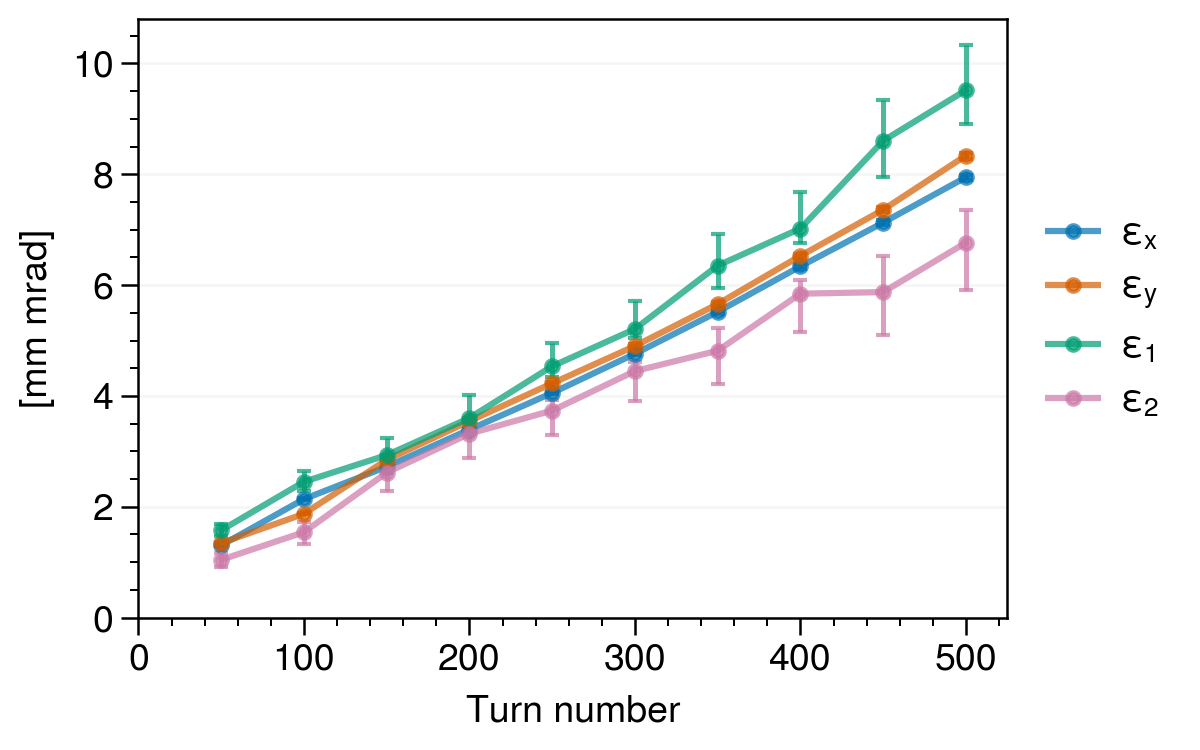
\includegraphics[width=\textwidth]{Images/chapter5/exp2/emittances.png}
    \end{subfigure}
    \vfill
    \vspace*{-0.2cm}
    \vfill
    \begin{subfigure}{0.8\textwidth}
        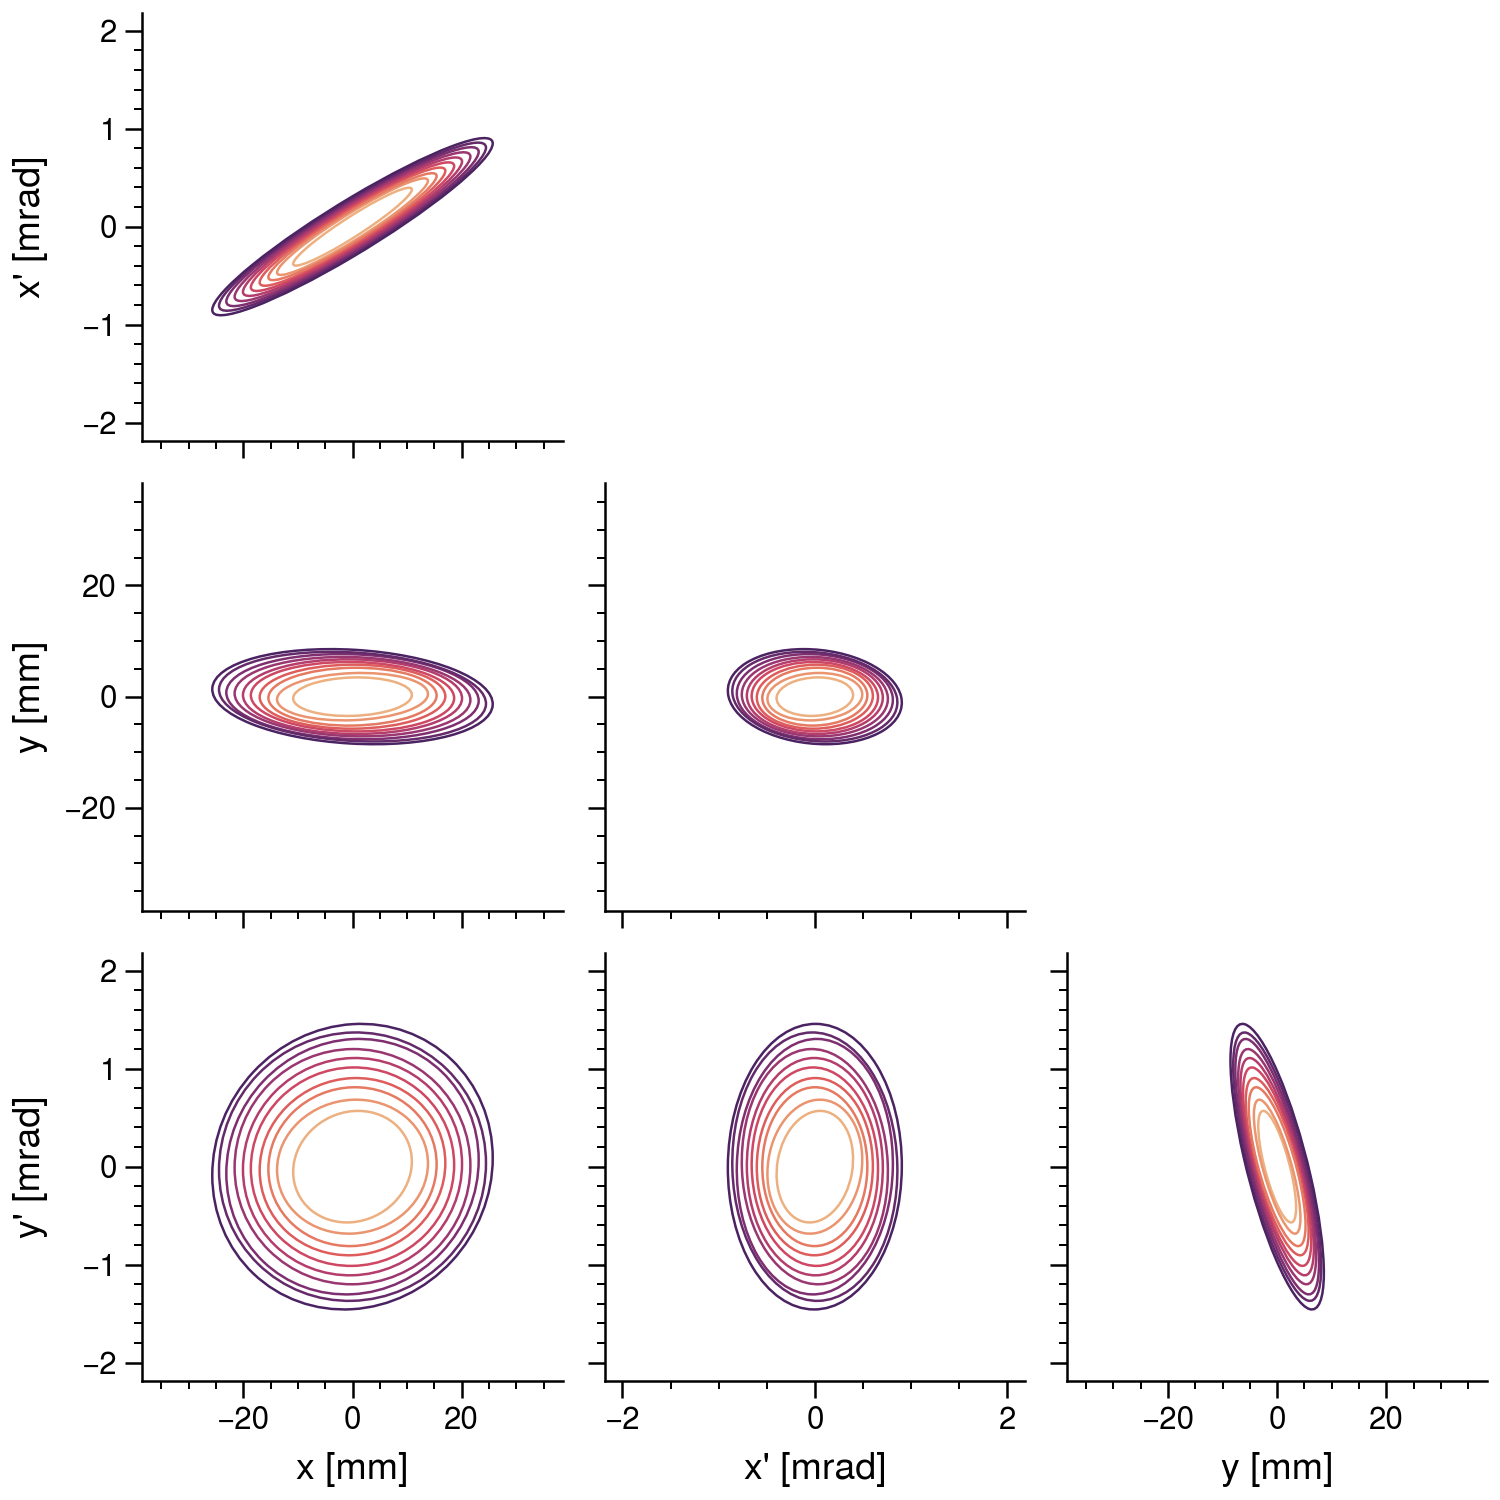
\includegraphics[width=\textwidth]{Images/chapter5/exp2/corner.png}
    \end{subfigure}
    \caption{Reconstructed emittances and covariance ellipses of a 0.8 GeV beam during injection. Initial injected coordinates: ($x$, $x'$, $y$, $y'$) $\approx$ (0 mm, 0 mrad, 0 mm, 0 mrad). Final injected coordinates: ($x$, $x'$, $y$, $y'$) $\approx$ (21 mm, 0 mrad, 0 mm, 1.1 mrad).}
    \label{fig:exp2_emittances}
\end{figure}
%

\section{Experiment 3}


%
\begin{figure}[!p]
    \centering
    \begin{subfigure}{\textwidth}
        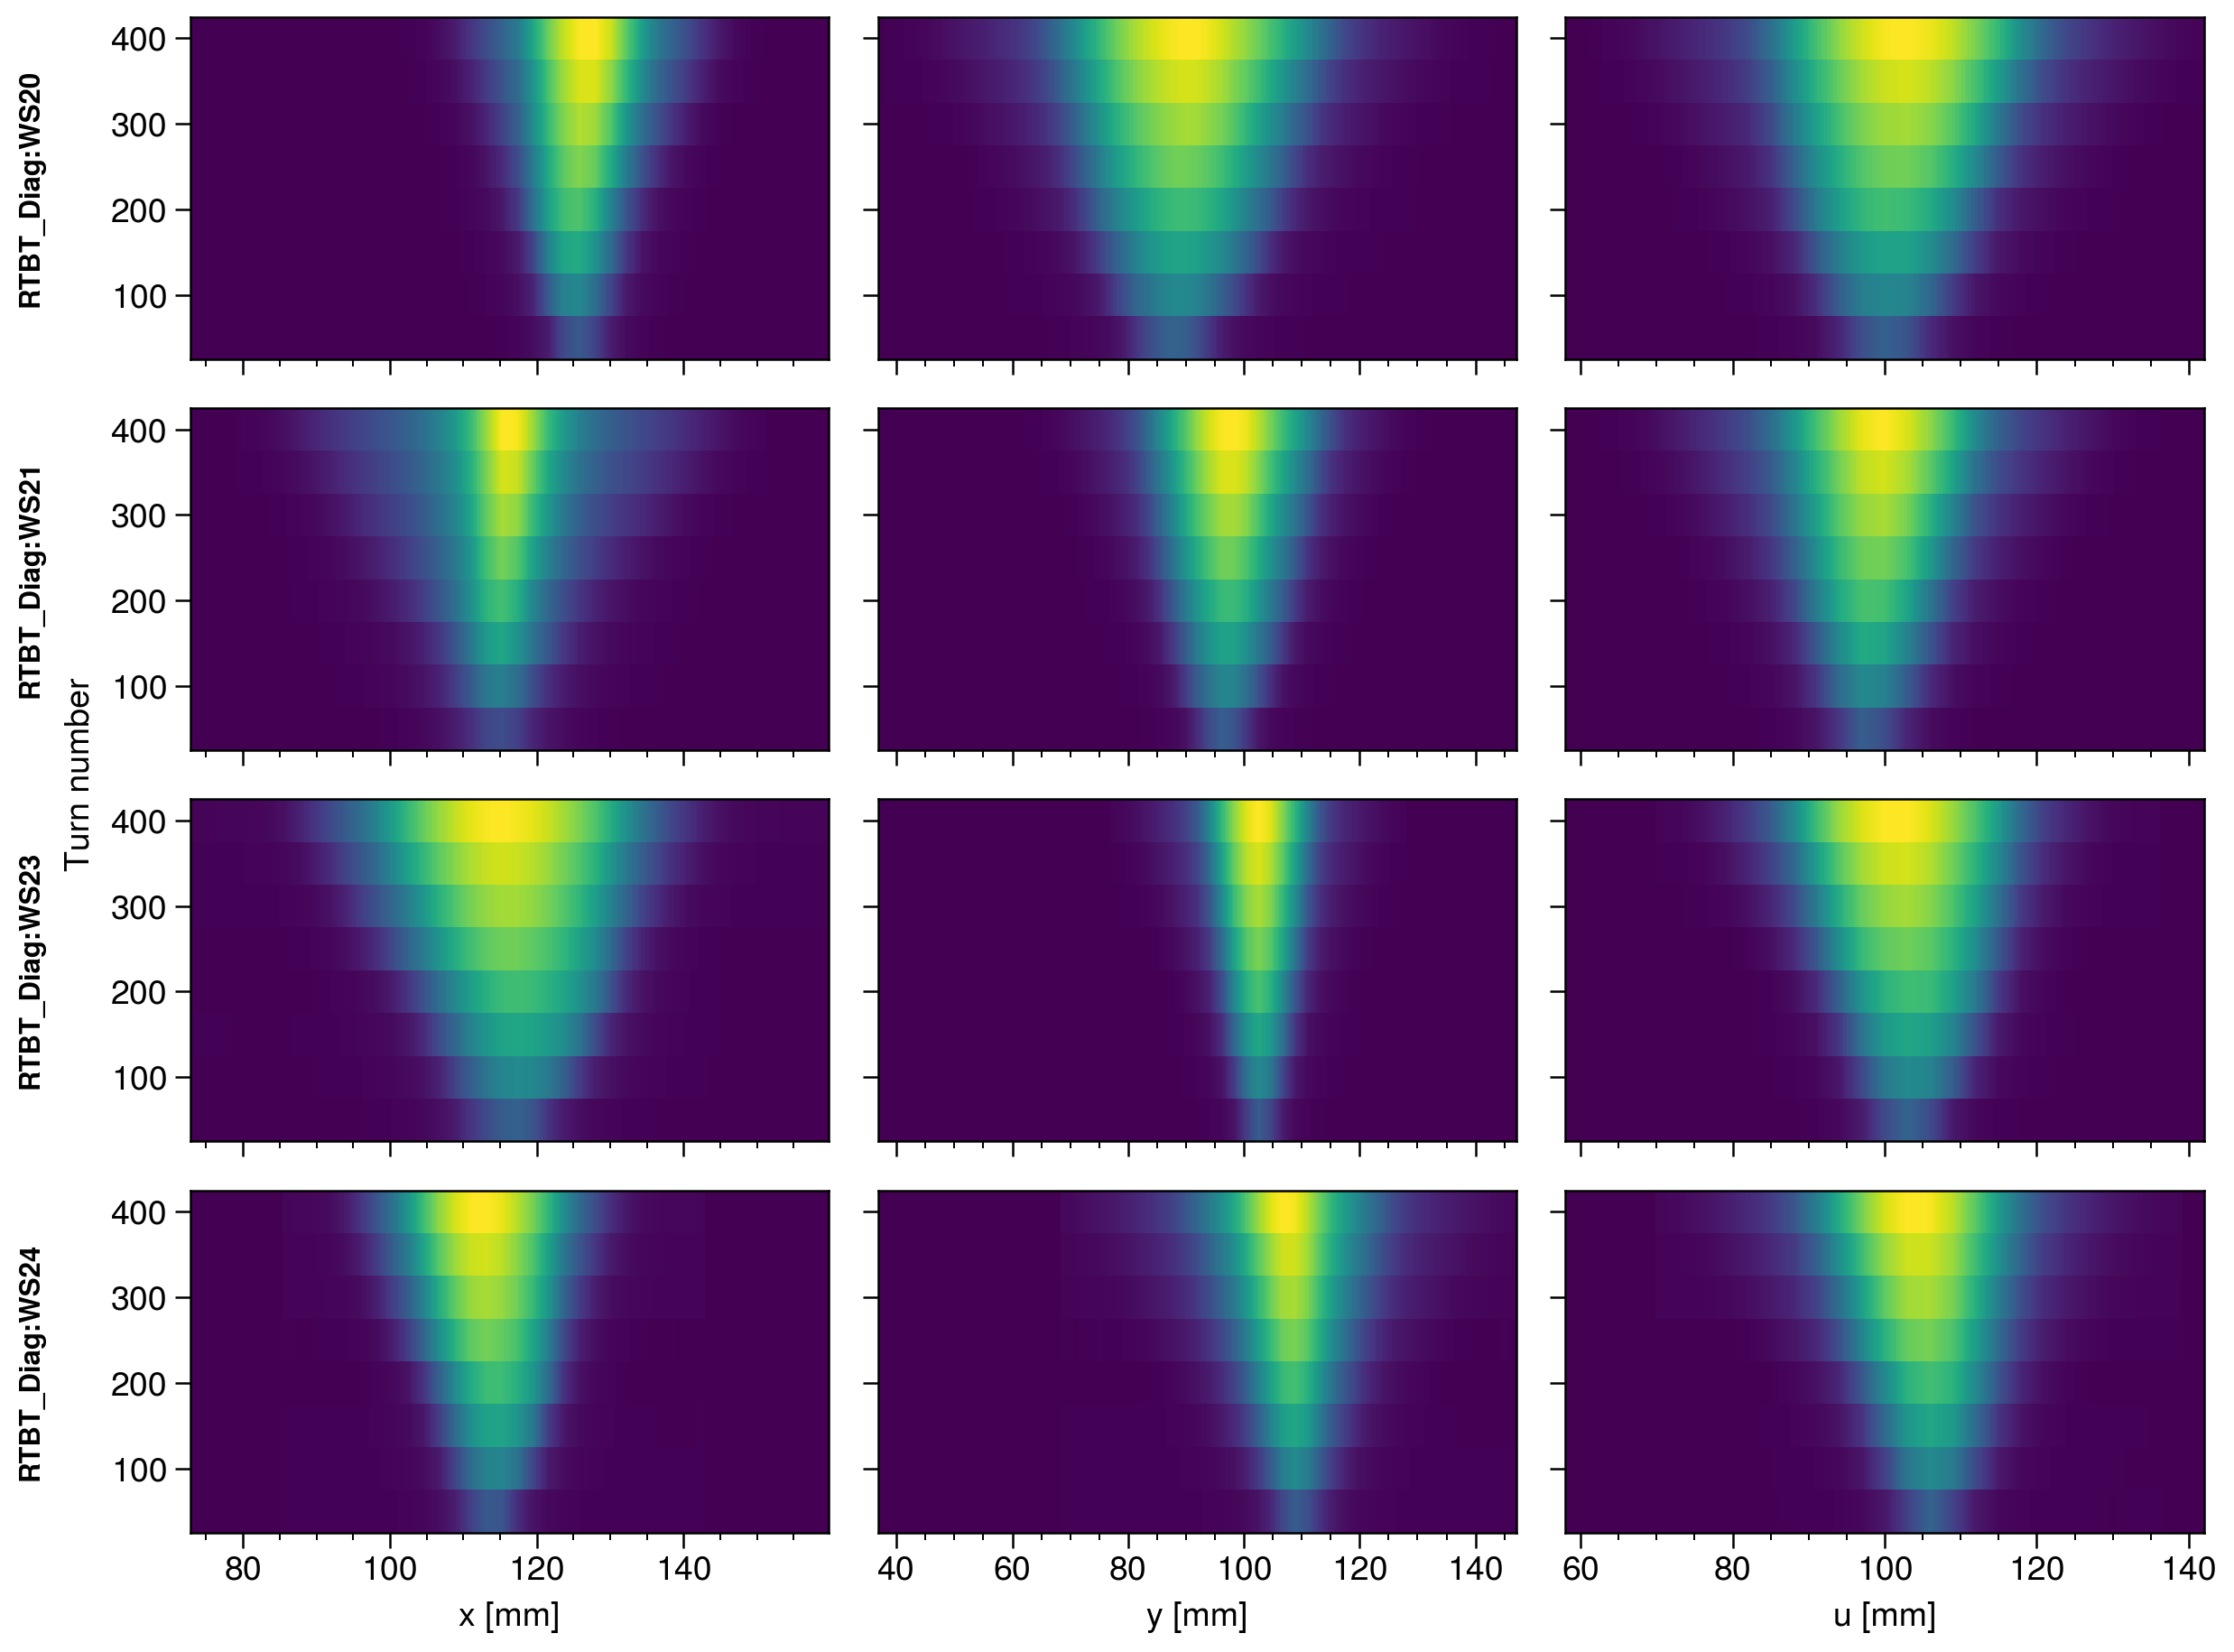
\includegraphics[width=\textwidth]{Images/chapter5/exp3/waterfall.png}
    \end{subfigure}
    \vfill
    \vspace*{1.25cm}
    \vfill
    \begin{subfigure}{\textwidth}
        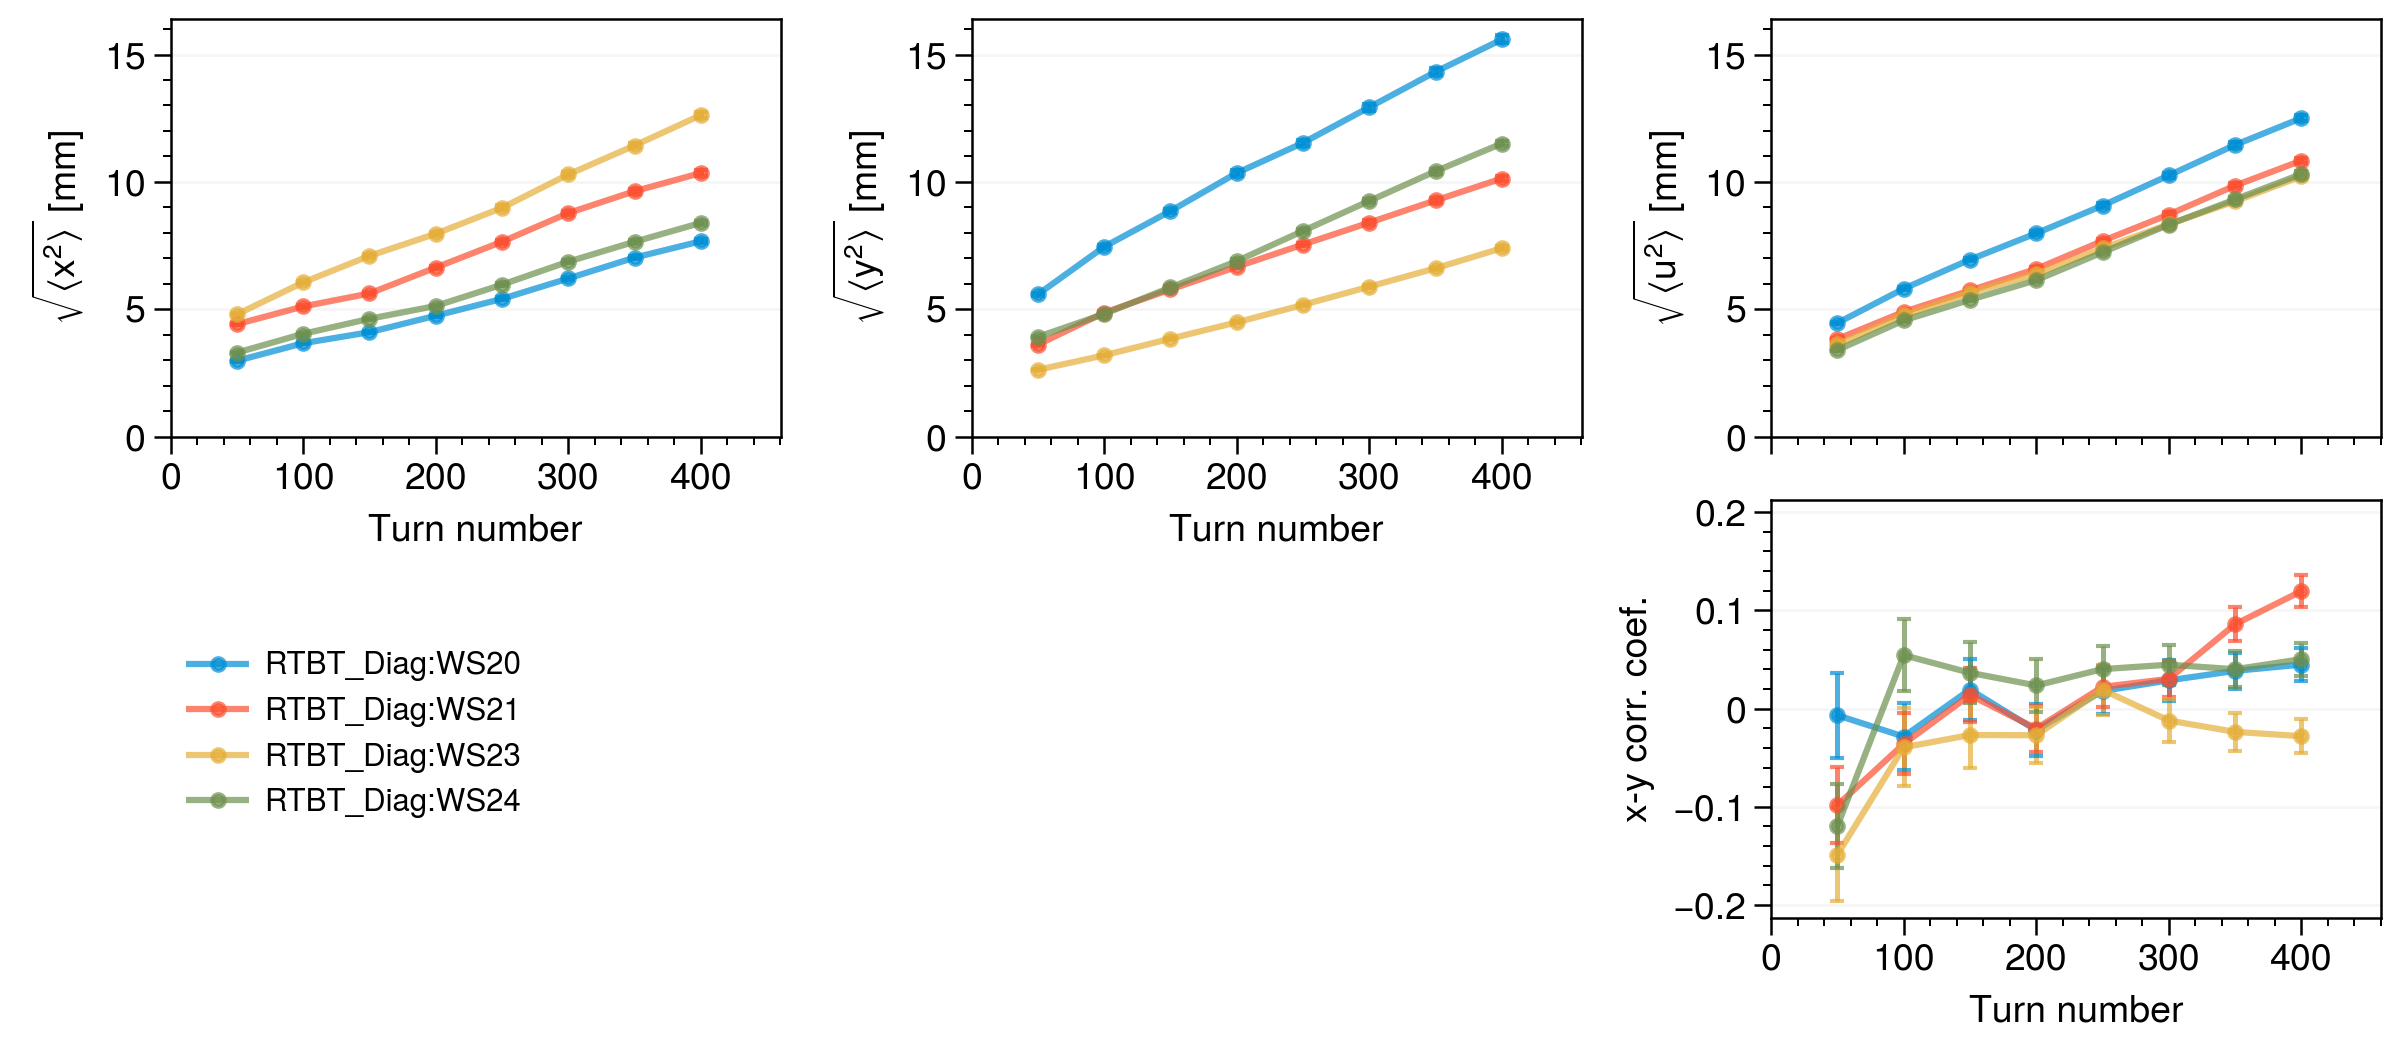
\includegraphics[width=\textwidth]{Images/chapter5/exp3/rms.png}
    \end{subfigure}
    \caption{Measured wire-scanner profiles during injection for a 0.8 GeV beam. Initial injected coordinates: ($x$, $x'$, $y$, $y'$) $\approx$ (0 mm, 0 mrad, 0 mm, 0 mrad). Final injected coordinates: ($x$, $x'$, $y$, $y'$) $\approx$ (31 mm, 0 mrad, 0 mm, 1.1 mrad).}
    \label{fig:exp3_wsmeas}
\end{figure}
%

%
\begin{figure}[!p]
    \centering
    \begin{subfigure}{0.6\textwidth}
        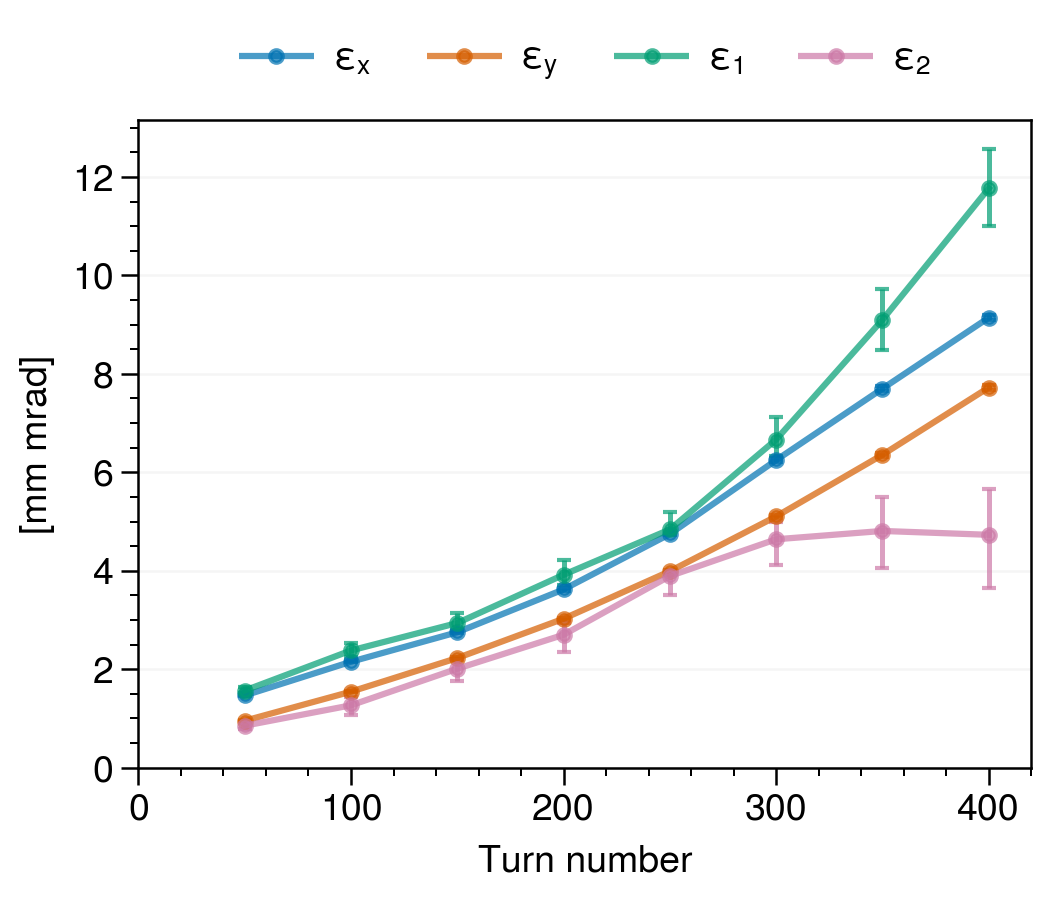
\includegraphics[width=\textwidth]{Images/chapter5/exp3/emittances.png}
    \end{subfigure}
    \vfill
    \vspace*{-0.2cm}
    \vfill
    \begin{subfigure}{0.8\textwidth}
        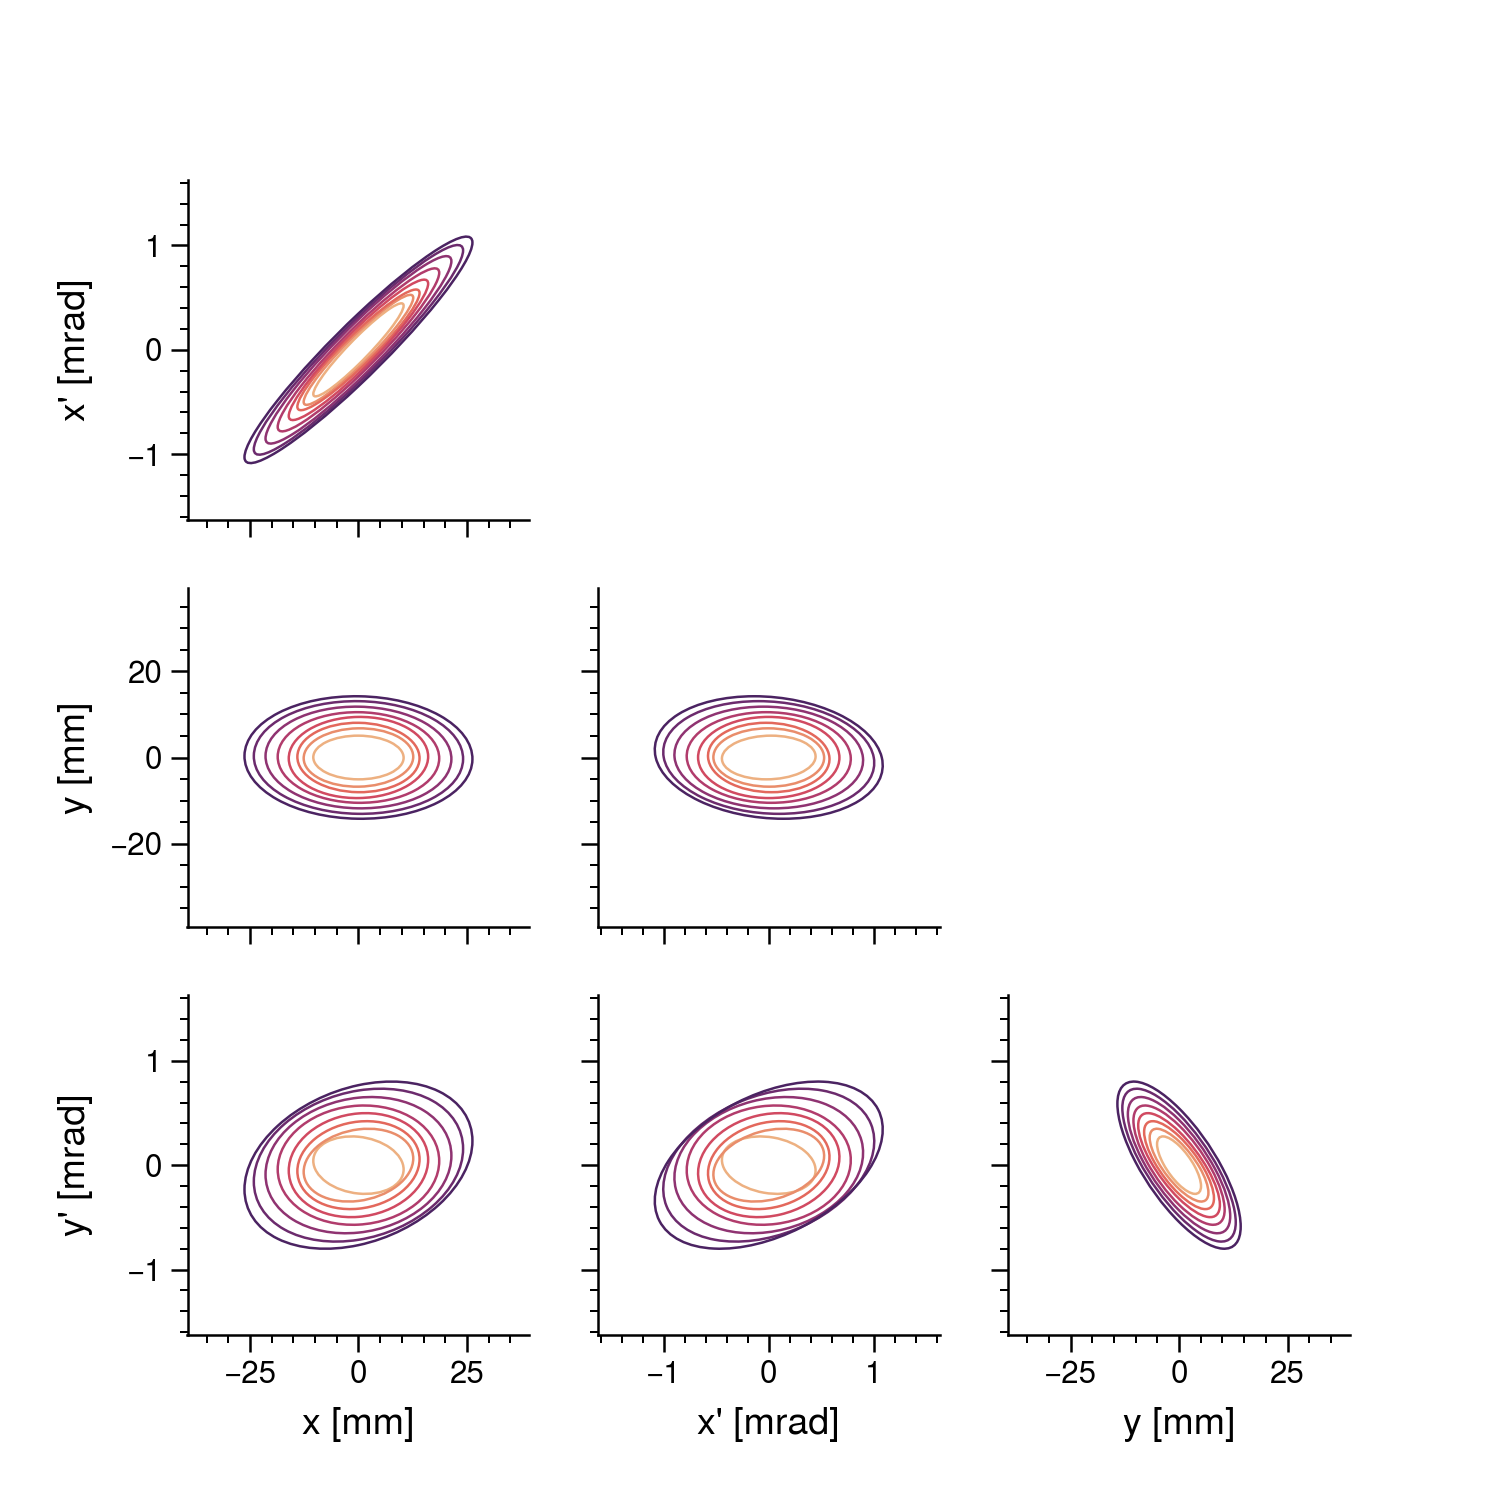
\includegraphics[width=\textwidth]{Images/chapter5/exp3/corner.png}
    \end{subfigure}
    \caption{Reconstructed emittances and covariance ellipses of a 0.8 GeV beam during injection. Initial injected coordinates: ($x$, $x'$, $y$, $y'$) $\approx$ (0 mm, 0 mrad, 0 mm, 0 mrad). Final injected coordinates: ($x$, $x'$, $y$, $y'$) $\approx$ (31 mm, 0 mrad, 0 mm, 1.1 mrad).}
    \label{fig:exp3_emittances}
\end{figure}
%



\section{Experiment 4}



\section{Summary}